%!TEX ROOT = thesis.tex

\chapter{Vehicle Semantics Retrieval Engine}

\label{section:retrievalengine}
\section{Introduction}

As described in Section~\ref{section:introduction}, there is an evident gap between the process of obtaining user described events and the retrieval of the desired video shots. Traditional approaches of collecting text-based description of events alone are both insufficient and somewhat impractical for the retrieval process.
With vehicle-specific semantics such as vehicle trajectory, time-stamp information, and colour information extracted via the extraction module described in Chapter~\ref{section:semanticsextraction}, this chapter discusses on achieving the second objective [O2] of designing video retrieval techniques that take in intuitive user-described queries, and provide fast and accurate results.

To this end, a keyword and sketch based retrieval engine was designed for end users to describe their queries intuitively. In this chapter, we first discuss the design choices of the semantic retrieval engines in detail. Two retrieval techniques with relatively different concepts and underlying frameworks were designed. 
The first technique was designed with a classic document retrieval system in mind, inspired by Locality Sensitive Hashing (LSH), while the second technique was developed in order to address the shortcomings of the first by introducing similarity scores obtained using Chamfer Distance.

Subsequently, the methods used to measure the difference between the
trajectories, vehicle colour classifying methods, scoring systems and the results based on multiple user reviews are discussed in detail.
As described in the Experimental Methodology (in Section~\ref{sec:expmethodology}),
both the vehicle trajectory and vehicle colour evaluation process were separated in order to better gauge the performance of each technique individually.
This chapter also reports the retrieval speed of the second retrieval engine for a quantitative measure of its efficiency.
The evaluation and analysis of their performances along with the metrics used are also discussed. This chapter concludes with some
suggestions for future improvements.

\section{\versionOneRet}
\label{section:versionOne}
This section covers the techniques used in this retrieval engine
framework together with corresponding results. As previously introduced, this retrieval engine is inspired by Locality Sensitive Hashing (LSH), a technique where documents are hashed into similar locations depending on their similarity with one another. 
%With that, the concept of this retrieval engine is first discussed. Next, the scoring system is introduced followed by the evaluation of the system in the following subsections.

\subsection{Concept}
\label{versionOneConcept}
By taking advantage of the spatio-temporal atom cubes structure introduced in
Chapter~\ref{section:atoms}, each catalogued event %in an atom 
is treated as a
unique \emph{document}, using retrieval terminology. The underlying atom-based structure allows queries to be formed in a manner which emulates the semantics extraction process. Hence, this eliminates the need for query parsing which in turn reduces the required computational time.

In this setup, each document containing similar contents are expected to be placed in the same data store as a mode of clustering documents. An example is given in
Table~\ref{table:dbSample} to provide a clear depiction of the proposed
method. These sequences of events is also visualised in
Figure~\ref{fig:motionExample} with the trajectory marked with \textcircled{2}.
In the example, a red vehicle was detected from frame 180 to 184 of a video file on the 19th of March 2016 (`20160319') from 8:51:00am until 8:51:05am (within the 6-minute file named with timestamp `084800'), from atom location (3, 15)
to (5, 17) but was detected as a pink vehicle at frame 181.
The time information from frame $\mathbb{T}$ can be deduced using Equation \ref{eq:timecount}.
%$\mathbb{T}_{time}  = (\mathbb{VD} \times \frac{\mathbb{T}}{\mathbb{TF}}) + \mathbb{F}_{time}$
%where $\mathbb{VD}$ corresponds to the video duration of each file (6 minutes)
%and $\mathbb{TF}$ is the total frames of the current video. The
%$\mathbb{F}_{time}$ is the time information extracted from filename. 
Hence, in this example, the
current frame time at frame 181 is obtained as such: Adding $(6_{minutes}$ $\times$ $\frac{181}{360})$ to 08:48:00am $\rightarrow$ 8:51:01am.

As each catalogued event is treated as a unique document (a single record in the database) in this framework, the implementation of the retrieval process works by filtering out parts of the record store
%tables 
that are irrelevant to the query, $\mathbb{Q}$. In the same example given in Table~\ref{table:dbSample}, the retrieval engine is able to effectively
skip through 9 colour tables and 5 motion tables, hence speeding up the process of locating documents of interest while reducing the overhead cost involved when going through an entire database. Upon filtering out irrelevant tables,
the retrieval engine proceeds to extract and group all the relevant records according to the filenames.

Next, the retrieved results are validated to see if they belong to the same vehicle by cross-checking the \emph{obj\_id} field. Along with that, the retrieval engine also validates if the results belong to a similar time-frame by comparing the $t$-coordinates. This step is essential to ensure that each result belongs to the same vehicle trajectory group as the initial tracker may re-assign a \emph{obj\_id} to another vehicle during the earlier background subtraction process. Although the results returned at this point are moderately accurate, one major problem that occurs using the current process is the low recall rate. The recall rate in a retrieval task is given as the percentage of relevant
documents retrieved over the total amount of relevant documents available in the database. While low recall rates might be preferable in an environment where the accuracy of the retrieved result is of higher importance and false negatives are welcomed over false positives such as in medical applications, this
is not the case for this particular problem.

To overcome the limitation of low recall rates, a Confidence Value ($CV$) score is introduced to adjust the sensitivity level of accepting a video shot as part of the final retrieved results. Intuitively, a lower $CV$ would return a larger set of results at the expense of an increase of retrieved shots which may or may not improve the overall accuracy. Each retrieved shot, $\mathbb{S}_i$, will be accepted as the final retrieved results if it fulfils
the condition in Equation \ref{eq:CVscore}. The use of the $CV$ score parameter provides a margin of error when performing the query which acts as a trade-off factor.
\begin{equation}
\label{eq:CVscore}
CV < \frac{\text{length}(\mathbb{S}_i)}{\text{length}(\mathbb{Q})} \times 100\%
\end{equation}

Upon validating the results, %commands were sent to FFmpeg to extract 
the matching video shots are extracted based on the given filename along with the start and end frame number. Finally, the implemented system presents users with the output from the retrieval engine where the final results can be viewed via the same interface.


% Please add the following required packages to your document preamble:
% \usepackage[normalem]{ulem}
\begin{table}[tb!]
	\centering
  \caption{Atom Records of a Sample Red Vehicle in the Data Store. %Identified as Red and Pink Colour
  %with Object ID ``1'' of the \versionOneRet
  }
  \label{table:dbSample}
  \begin{tabular}{llllll}
  \multicolumn{6}{l}{{ colour\_red}} \\ \hline
  \multicolumn{1}{|l|}{\textbf{row\_id}} & \multicolumn{1}{l|}{\textbf{filename}}    & \multicolumn{1}{l|}{\textbf{obj\_id}} & \multicolumn{1}{l|}{\textbf{atom\_x}} & \multicolumn{1}{l|}{\textbf{atom\_y}} & \multicolumn{1}{l|}{\textbf{atom\_t}} \\ \hline
  \multicolumn{1}{|l|}{n}                & \multicolumn{1}{l|}{20160319\_084800.mp4} & \multicolumn{1}{l|}{1}                & \multicolumn{1}{l|}{3}                & \multicolumn{1}{l|}{15}               & \multicolumn{1}{l|}{180}              \\ \hline
  \multicolumn{1}{|l|}{n+1}              & \multicolumn{1}{l|}{20160319\_084800.mp4} & \multicolumn{1}{l|}{1}                & \multicolumn{1}{l|}{3}                & \multicolumn{1}{l|}{16}               & \multicolumn{1}{l|}{182}              \\ \hline
  \multicolumn{1}{|l|}{n+2}              & \multicolumn{1}{l|}{20160319\_084800.mp4} & \multicolumn{1}{l|}{1}                & \multicolumn{1}{l|}{4}                & \multicolumn{1}{l|}{16}               & \multicolumn{1}{l|}{183}              \\ \hline
  \multicolumn{1}{|l|}{n+3}              & \multicolumn{1}{l|}{20160319\_084800.mp4} & \multicolumn{1}{l|}{1}                & \multicolumn{1}{l|}{5}                & \multicolumn{1}{l|}{17}               & \multicolumn{1}{l|}{184}              \\ \hline
                                         &                                           &                                       &                                       &                                       &                                       \\
  \multicolumn{6}{l}{{ colour\_pink}}                                                                                                                                                                                                              \\ \hline
  \multicolumn{1}{|l|}{\textbf{row\_id}} & \multicolumn{1}{l|}{\textbf{filename}}    & \multicolumn{1}{l|}{\textbf{obj\_id}} & \multicolumn{1}{l|}{\textbf{atom\_x}} & \multicolumn{1}{l|}{\textbf{atom\_y}} & \multicolumn{1}{l|}{\textbf{atom\_t}} \\ \hline
  \multicolumn{1}{|l|}{m}                & \multicolumn{1}{l|}{20160319\_084800.mp4} & \multicolumn{1}{l|}{1}                & \multicolumn{1}{l|}{3}                & \multicolumn{1}{l|}{16}               & \multicolumn{1}{l|}{181}              \\ \hline
                                         &                                           &                                       &                                       &                                       &                                       \\
  \multicolumn{6}{l}{{ direction\_down}}                                                                                                                                                                                                          \\ \hline
  \multicolumn{1}{|l|}{\textbf{row\_id}} & \multicolumn{1}{l|}{\textbf{filename}}    & \multicolumn{1}{l|}{\textbf{obj\_id}} & \multicolumn{1}{l|}{\textbf{atom\_x}} & \multicolumn{1}{l|}{\textbf{atom\_y}} & \multicolumn{1}{l|}{\textbf{atom\_t}} \\ \hline
  \multicolumn{1}{|l|}{h}                & \multicolumn{1}{l|}{20160319\_084800.mp4} & \multicolumn{1}{l|}{1}                & \multicolumn{1}{l|}{3}                & \multicolumn{1}{l|}{15}               & \multicolumn{1}{l|}{181}              \\ \hline
                                         &                                           &                                       &                                       &                                       &                                       \\
  \multicolumn{6}{l}{{ direction\_motionless}}                                                                                                                                                                                                    \\ \hline
  \multicolumn{1}{|l|}{\textbf{row\_id}} & \multicolumn{1}{l|}{\textbf{filename}}    & \multicolumn{1}{l|}{\textbf{obj\_id}} & \multicolumn{1}{l|}{\textbf{atom\_x}} & \multicolumn{1}{l|}{\textbf{atom\_y}} & \multicolumn{1}{l|}{\textbf{atom\_t}} \\ \hline
  \multicolumn{1}{|l|}{j}                & \multicolumn{1}{l|}{20160319\_084800.mp4} & \multicolumn{1}{l|}{1}                & \multicolumn{1}{l|}{3}                & \multicolumn{1}{l|}{16}               & \multicolumn{1}{l|}{182}              \\ \hline
                                         &                                           &                                       &                                       &                                       &                                       \\
  \multicolumn{6}{l}{{ direction\_right}}                                                                                                                                                                                                         \\ \hline
  \multicolumn{1}{|l|}{\textbf{row\_id}} & \multicolumn{1}{l|}{\textbf{filename}}    & \multicolumn{1}{l|}{\textbf{obj\_id}} & \multicolumn{1}{l|}{\textbf{atom\_x}} & \multicolumn{1}{l|}{\textbf{atom\_y}} & \multicolumn{1}{l|}{\textbf{atom\_t}} \\ \hline
  \multicolumn{1}{|l|}{k}                & \multicolumn{1}{l|}{20160319\_084800.mp4} & \multicolumn{1}{l|}{1}                & \multicolumn{1}{l|}{3}                & \multicolumn{1}{l|}{16}               & \multicolumn{1}{l|}{183}              \\ \hline
                                         &                                           &                                       &                                       &                                       &                                       \\
  \multicolumn{6}{l}{{ direction\_right\_down}}                                                                                                                                                                                                   \\ \hline
  \multicolumn{1}{|l|}{\textbf{row\_id}} & \multicolumn{1}{l|}{\textbf{filename}}    & \multicolumn{1}{l|}{\textbf{obj\_id}} & \multicolumn{1}{l|}{\textbf{atom\_x}} & \multicolumn{1}{l|}{\textbf{atom\_y}} & \multicolumn{1}{l|}{\textbf{atom\_t}} \\ \hline
  \multicolumn{1}{|l|}{l}                & \multicolumn{1}{l|}{20160319\_084800.mp4} & \multicolumn{1}{l|}{1}                & \multicolumn{1}{l|}{3}                & \multicolumn{1}{l|}{16}               & \multicolumn{1}{l|}{184}              \\ \hline
  \end{tabular}
\end{table}

\subsection{Search Interface}

The proposed retrieval engine was presented in a graphical user interface (GUI) written in C++. This way, users are able to construct queries by drawing the trajectory on the search interface while providing complementary query information such as vehicle colour and time period. Given a user-described query, the retrieval engine would search for the best matches and return the results within seconds. Figure \ref{fig:versionOneInterface} shows the proposed search interface with the green lines indicating the user-described trajectory query. Upon processing the results, video shots are extracted and the results are populated in a folder.
\begin{figure}[!tb]
	\centering
	\begin{tabular}{c}
		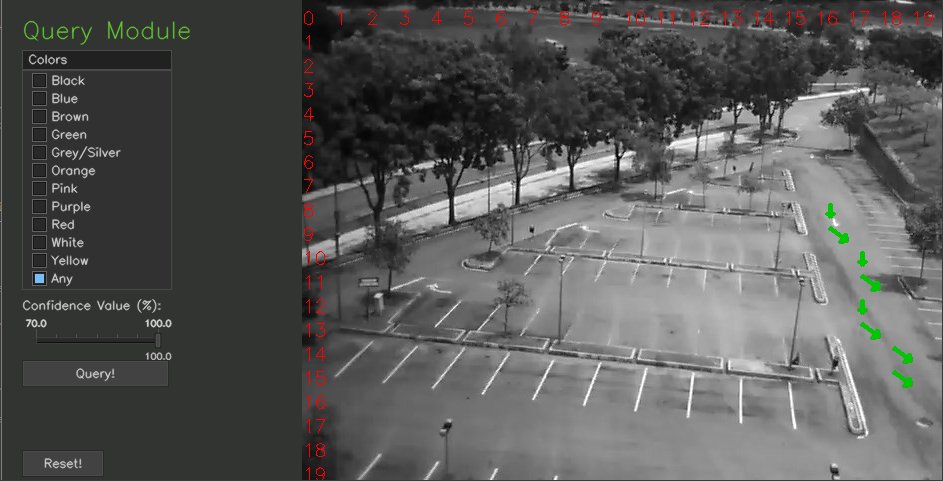
\includegraphics[width=0.7\linewidth]{image/retrievalOne/test1-8inputs.PNG} \\
		(a) Motion Test Case 1 (TQ1) \\
		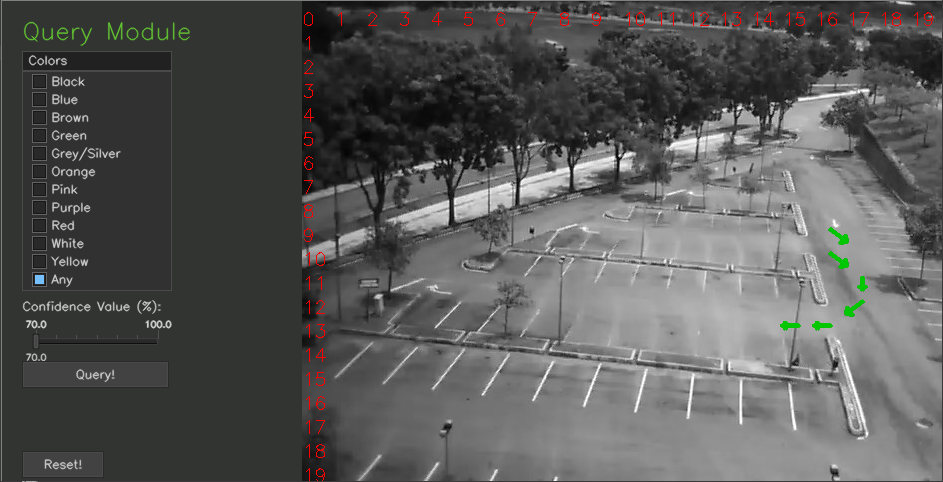
\includegraphics[width=0.7\linewidth]{image/retrievalOne/test2-6input.PNG}\\
		(b) Motion Test Case 2 (TQ2)
	\end{tabular}
	\caption{Search Interface for \versionOneRet}
	\label{fig:versionOneInterface}
\end{figure}

\subsection{Results and Analysis}
The following subsections describe the evaluation process of the proposed method in Section \ref{section:semantic_lsh} which includes both the vehicle trajectory as well as the vehicle colour. As previously mentioned in Section \ref{sec:expmethodology}, in this initial experiment, only two days of data were fully annotated with vehicles and their corresponding colours (see Table
\ref{table:colorDist}) as well as the total number of vehicles that performed two pre-determined test queries (TQ1 and TQ2).

Precision and Recall (Equation \ref{eq:precisionrecall}) metrics are used to measure the performance of the proposed method. These values are calculated based on the total number of annotated events that occurred over the designated 2-day period.
Likewise, as the $F_1$-Score is a harmonic mean between Precision and Recall, this value can be computed as in Equation \ref{eq:f1score}. The precision of a retrieval engine is the ratio between number of accurate results over the total number of retrieved results. The recall, on the hand, indicates the ratio of relevant results which were retrieved over the total retrieved results. As both high Precision and Recall values are equally desirable in a retrieval
engine, the $F_1$-Score is used to judge how well the retrieval engine performs with both aspects taken into consideration.
\begin{align}
\label{eq:precisionrecall}
    \text{Precision} = \frac{tp}{tp + fp}   \hspace{1em} \text{ ; }  \hspace{1em} \text{Recall}  = \frac{tp}{tp + fn}
\end{align}
\begin{align}
\label{eq:f1score}
F_{1}-\text{score}  = 2\cdot\frac{\text{Precision} \cdot \text{Recall}}{\text{Precision} + \text{Recall}}
\end{align}

\subsubsection{Vehicle Trajectory}

To evaluate the performance of the proposed method in retrieving vehicle trajectories, the ground truth data has to be first obtained. As the manual annotation of these video data is laborious and time consuming, only two specific motion paths were designated as trajectory queries (TQ). The first query, TQ1 refers to vehicles heading southwards (see Figure
\ref{fig:versionOneInterface} (a)) while TQ2 represents vehicles turning into
a junction (see Figure \ref{fig:versionOneInterface} (b)).

These predefined trajectory queries (TQ) were selected to represent two types
of motion which are common in a typical car park scene: (i) \textit{simple
motion} - motions that are simple in nature, moving straight \& (ii)
\textit{complex motion} - motions which contains two or more motion elements
such as turning into a junction. The distribution of these TQs are tabulated in Table \ref{table:motiondist}. In each TQ experiment, the number of atoms selected in the input queries were varied to understand the relation between the number of inputs and the performance of the retrieval engine. In addition, the effects of using varying confidence values (CV) is also evaluated. These experiments were tested on three CV values which were set at 70\%, 80\%, and 90\%.
\begin{table}[tb!]
\centering
  \caption{Ground Truth Distribution of Trajectory Query Types}
\label{table:motiondist}
\begin{tabular}{cccc}
\toprule
Trajectory Query &  Trajectory Type & \# of Occurrence & Distribution (\%)   \\
\midrule
TQ1       & Simple Motion       & 252 & 86.3   \\
TQ2      & Complex Motion       & 40 & 13.7  \\
\bottomrule
\end{tabular}
\end{table}
\begin{table}[tb!]
\centering
\caption{Results of Motion Retrieval Task with Varying Confidence Value and
  Number of Atom Inputs}
\label{table:motionResults}
\vspace{0.5em}
\resizebox{\textwidth}{!}{
\begin{tabular}{ccc|c|c|c|c|c|c|c|c|c|}
\cline{4-12}
\cline{4-12}
& & & \multicolumn{3}{c|}{CV: 70\%} & \multicolumn{3}{c|}{CV: 80\%} & \multicolumn{3}{c|}{CV: 90\%} \\ \cline{4-12}
 & & & Precision & Recall & F1 Score & Precision & Recall & F1 Score & Precision & Recall & F1 Score \\ \hline
\multicolumn{1}{|c|}{\multirow{7}{*}{\rotatebox[origin=c]{90}{No. of Inputs}}} & \multicolumn{1}{c|}{\multirow{4}{*}{\rotatebox[origin=c]{90}{TQ1}}} & 5 & 93.82 & 61.53  & \cellcolor[HTML]{32CB00}\textbf{74.32} & 95.34 & 33.19  & 49.24 & 95.34 & 33.19 & 49.24   \\ \cline{3-12}
\multicolumn{1}{|c|}{} & \multicolumn{1}{c|}{} & 6 & 90.09 & 36.84 & 52.29 & 90.09 & 36.84  & 52.29 & 89.13 & 16.59 & 27.98    \\ \cline{3-12}
\multicolumn{1}{|c|}{} & \multicolumn{1}{c|}{} & 7 & 87.27 & 38.86 & 53.78 & 88 & 17.81  & 29.62 & 87.87 & 11.74 & 20.71    \\ \cline{3-12}
\multicolumn{1}{|c|}{} & \multicolumn{1}{c|}{} & 8 & 86.88 & 21.45 & 34.41 & 84.61 & 13.36  & 23.07 & 89.65 & 10.52 & 18.84    \\ \cline{2-12}
\multicolumn{1}{|c|}{} & \multicolumn{1}{c|}{\multirow{3}{*}{\rotatebox[origin=c]{90}{TQ2}}} & 4 & 16.28 & 80 & 27.06 & 28.69 & 73.33  & 41.25    & 28.69 & 73.33 & 41.25    \\ \cline{3-12}
\multicolumn{1}{|c|}{} & \multicolumn{1}{c|}{} & 5 & 65.3 & 71.11  & \cellcolor[HTML]{32CB00}\textbf{68.08} & 73.33 & 48.88  & 58.66 & 73.33 & 48.88  & 58.66    \\ \cline{3-12}
\multicolumn{1}{|c|}{} & \multicolumn{1}{c|}{} & 6 & 55.81 & 53.33 & 54.54 & 55.81 & 53.33 & 54.54 & 57.69 & 33.33 & 42.25    \\ \hline
\end{tabular}}
\end{table}

Based on the results tabulated in Table \ref{table:motionResults}, the average
precision (AP) for both TQ1 and TQ2 using CV at 70\% is 67.64\%. The increase in CV from 70\% to 90\% shows an increase in terms of average precision. For TQ1, the
average precision increased from 89.50\% to 90.49\% when CV was set at 90\%
with an increase of approximately 1\%. However for TQ2, the average
precision showed a sizeable improvement of 7.44\% when the CV parameter increases, \emph{i.e.} from 45.79\% to 53.23\% when CV changed from 70\% to 90\%.
However, as expected, the recall metrics showed a different side of the story: the average recall (AR) rate suffered a drastic drop from 39.67\% to 18.01\%
for TQ1 and 68.15\% to 51.85\% for TQ2. Overall, the results shows consistency
throughout the various experimental settings and is a reflection of the concept which was introduced in \ref{versionOneConcept}.

To judge the overall performance of the retrieval engine as a whole, the $F_1$-Score metric is a desirable metric. %as it provides a harmonic mean between both of the desirable metrics discussed above. 
Based on the results, queries with the lowest CV and a lower number of input atoms tend to perform better than other combination of parameter settings.
This is an expected behaviour because the additional number of inputs increases the chance of incorrect matches. Likewise, a lower CV value relaxes the need to match more atom
inputs.
The proposed method was able to achieve an $F_1$-Score of 74.32\% and 68.08\% for both TQ1 and TQ2 using the most desirable parameters. Based on the results obtained from these experiments, the performance of the proposed method is still far from optimal. %Drastic changes are inevitable if improvements is desired. 
Further improvements to the proposed method will be discussed in Section \ref{section:versionTwo}.

\begin{table}[tb!]
\centering
\caption{Ground Truth Distribution Vehicle Colours Ordered by Occurrence}
\label{table:colorDist}
\begin{tabular}{ccc}
\toprule
Colour Term & \# of Occurrence & Distribution (\%)   \\
\midrule
Gray       & 365       & 43.61  \\
Black      & 182       & 21.74  \\
White      & 150       & 17.92  \\
Red        & 60        & 7.17   \\
Blue       & 19        & 2.27   \\
Orange     & 15        & 1.79   \\
Yellow     & 13        & 1.55   \\
Green      & 10        & 1.19   \\
Pink       & 9         & 1.08   \\
Purple     & 7         & 0.84   \\
Brown      & 7         & 0.84   \\
\bottomrule
\end{tabular}
\end{table}
\begin{table}[tb!]
\centering
\caption{Confusion Matrix for Colour Retrieval Task}
\label{table:colorMatrix}
\resizebox{\columnwidth}{!}{
\begin{tabular}{ccccccccccccc}
\cline{3-13}
 & \multicolumn{1}{l|}{} & \multicolumn{11}{c|}{Predicted Colour} \\ \cline{3-13}
 & \multicolumn{1}{c|}{} & \multicolumn{1}{c|}{Gray} & \multicolumn{1}{c|}{Black} & \multicolumn{1}{c|}{White} & \multicolumn{1}{c|}{Red} & \multicolumn{1}{c|}{Blue} & \multicolumn{1}{c|}{Orange} & \multicolumn{1}{c|}{Yellow} & \multicolumn{1}{c|}{Green} & \multicolumn{1}{c|}{Pink} & \multicolumn{1}{c|}{Purple} & \multicolumn{1}{c|}{Brown} \\ \hline
\multicolumn{1}{|l|}{} & \multicolumn{1}{c|}{Gray} & \multicolumn{1}{c|}{\cellcolor[HTML]{32CB00}\textbf{236}} & \multicolumn{1}{c|}{61} & \multicolumn{1}{c|}{68} & \multicolumn{1}{c|}{0} & \multicolumn{1}{c|}{0} & \multicolumn{1}{c|}{0} & \multicolumn{1}{c|}{0} & \multicolumn{1}{c|}{0} & \multicolumn{1}{c|}{0} & \multicolumn{1}{c|}{0} & \multicolumn{1}{c|}{0} \\ \cline{2-13}
\multicolumn{1}{|l|}{} & \multicolumn{1}{c|}{Black} & \multicolumn{1}{c|}{48} & \multicolumn{1}{c|}{\cellcolor[HTML]{32CB00}\textbf{134}} & \multicolumn{1}{c|}{0} & \multicolumn{1}{c|}{0} & \multicolumn{1}{c|}{0} & \multicolumn{1}{c|}{0} & \multicolumn{1}{c|}{0} & \multicolumn{1}{c|}{0} & \multicolumn{1}{c|}{0} & \multicolumn{1}{c|}{0} & \multicolumn{1}{c|}{0} \\ \cline{2-13}
\multicolumn{1}{|l|}{} & \multicolumn{1}{c|}{White} & \multicolumn{1}{c|}{26} & \multicolumn{1}{c|}{4} & \multicolumn{1}{c|}{\cellcolor[HTML]{32CB00}\textbf{120}} & \multicolumn{1}{c|}{0} & \multicolumn{1}{c|}{0} & \multicolumn{1}{c|}{0} & \multicolumn{1}{c|}{0} & \multicolumn{1}{c|}{0} & \multicolumn{1}{c|}{0} & \multicolumn{1}{c|}{0} & \multicolumn{1}{c|}{0} \\ \cline{2-13}
\multicolumn{1}{|l|}{} & \multicolumn{1}{c|}{Red} & \multicolumn{1}{c|}{27} & \multicolumn{1}{c|}{25} & \multicolumn{1}{c|}{0} & \multicolumn{1}{c|}{2} & \multicolumn{1}{c|}{0} & \multicolumn{1}{c|}{0} & \multicolumn{1}{c|}{0} & \multicolumn{1}{c|}{0} & \multicolumn{1}{c|}{4} & \multicolumn{1}{c|}{\cellcolor[HTML]{FE0000}\textbf{2}} & \multicolumn{1}{c|}{0} \\ \cline{2-13}
\multicolumn{1}{|l|}{} & \multicolumn{1}{c|}{Blue} & \multicolumn{1}{c|}{3} & \multicolumn{1}{c|}{10} & \multicolumn{1}{c|}{0} & \multicolumn{1}{c|}{0} & \multicolumn{1}{c|}{\cellcolor[HTML]{32CB00}\textbf{6}} & \multicolumn{1}{c|}{0} & \multicolumn{1}{c|}{0} & \multicolumn{1}{c|}{0} & \multicolumn{1}{c|}{0} & \multicolumn{1}{c|}{0} & \multicolumn{1}{c|}{0} \\ \cline{2-13}
\multicolumn{1}{|l|}{} & \multicolumn{1}{c|}{Orange} & \multicolumn{1}{c|}{8} & \multicolumn{1}{c|}{3} & \multicolumn{1}{c|}{0} & \multicolumn{1}{c|}{0} & \multicolumn{1}{c|}{0} & \multicolumn{1}{c|}{\cellcolor[HTML]{32CB00}\textbf{3}} & \multicolumn{1}{c|}{0} & \multicolumn{1}{c|}{0} & \multicolumn{1}{c|}{0} & \multicolumn{1}{c|}{1} & \multicolumn{1}{c|}{0} \\ \cline{2-13}
\multicolumn{1}{|l|}{} & \multicolumn{1}{c|}{Yellow}    & \multicolumn{1}{c|}{3} & \multicolumn{1}{c|}{1} & \multicolumn{1}{c|}{2} & \multicolumn{1}{c|}{0} & \multicolumn{1}{c|}{0} & \multicolumn{1}{c|}{0} & \multicolumn{1}{c|}{\cellcolor[HTML]{32CB00}\textbf{7}} & \multicolumn{1}{c|}{0} & \multicolumn{1}{c|}{0} & \multicolumn{1}{c|}{0} & \multicolumn{1}{c|}{0} \\ \cline{2-13}
\multicolumn{1}{|l|}{} & \multicolumn{1}{c|}{Green} & \multicolumn{1}{c|}{5} & \multicolumn{1}{c|}{1} & \multicolumn{1}{c|}{4} & \multicolumn{1}{c|}{0} & \multicolumn{1}{c|}{0} & \multicolumn{1}{c|}{0} & \multicolumn{1}{c|}{0} & \multicolumn{1}{c|}{\cellcolor[HTML]{C0C0C0}\textbf{0}} & \multicolumn{1}{c|}{0} & \multicolumn{1}{c|}{0} & \multicolumn{1}{c|}{0} \\ \cline{2-13}
\multicolumn{1}{|l|}{} & \multicolumn{1}{c|}{Pink} & \multicolumn{1}{c|}{1} & \multicolumn{1}{c|}{0} & \multicolumn{1}{c|}{0} & \multicolumn{1}{c|}{\cellcolor[HTML]{FE0000}\textbf{3}} & \multicolumn{1}{c|}{0} & \multicolumn{1}{c|}{0} & \multicolumn{1}{c|}{0} & \multicolumn{1}{c|}{0} & \multicolumn{1}{c|}{\cellcolor[HTML]{32CB00}\textbf{5}} & \multicolumn{1}{c|}{0} & \multicolumn{1}{c|}{0} \\ \cline{2-13}
\multicolumn{1}{|l|}{} & \multicolumn{1}{c|}{Purple} & \multicolumn{1}{c|}{3} & \multicolumn{1}{c|}{3} & \multicolumn{1}{c|}{0} & \multicolumn{1}{c|}{0} & \multicolumn{1}{c|}{0} & \multicolumn{1}{c|}{0} & \multicolumn{1}{c|}{0} & \multicolumn{1}{c|}{0} & \multicolumn{1}{c|}{0} & \multicolumn{1}{c|}{1} & \multicolumn{1}{c|}{0} \\ \cline{2-13}
\multicolumn{1}{|l|}{\multirow{-11}{*}{\rotatebox[origin=c]{90}{Actual Colour}}} & \multicolumn{1}{c|}{Brown} & \multicolumn{1}{c|}{3} & \multicolumn{1}{c|}{4} & \multicolumn{1}{c|}{0} & \multicolumn{1}{c|}{0} & \multicolumn{1}{c|}{0} & \multicolumn{1}{c|}{0} & \multicolumn{1}{c|}{0} & \multicolumn{1}{c|}{0} & \multicolumn{1}{c|}{0} & \multicolumn{1}{c|}{0} & \multicolumn{1}{c|}{\cellcolor[HTML]{C0C0C0}\textbf{0}} \\ \hline
 & \multicolumn{1}{l}{} & \multicolumn{1}{l}{} & \multicolumn{1}{l}{} & \multicolumn{1}{l}{} & \multicolumn{1}{l}{} & \multicolumn{1}{l}{} & \multicolumn{1}{l}{} & \multicolumn{1}{l}{} & \multicolumn{1}{l}{} & \multicolumn{1}{l}{} & \multicolumn{1}{l}{} & \multicolumn{1}{l}{} \\ \hline
\multicolumn{1}{|l|}{} & \multicolumn{1}{c|}{Precision} & \multicolumn{1}{c|}{65.01} & \multicolumn{1}{c|}{54.47}                                & \multicolumn{1}{c|}{61.86} & \multicolumn{1}{c|}{40.00} & \multicolumn{1}{c|}{100.00} & \multicolumn{1}{c|}{100.00}                             & \multicolumn{1}{c|}{100.00} & \multicolumn{1}{c|}{N/A} & \multicolumn{1}{c|}{55.56} & \multicolumn{1}{c|}{25.00}                              & \multicolumn{1}{c|}{N/A} \\ \cline{2-13}
\multicolumn{1}{|l|}{} & \multicolumn{1}{c|}{Recall} & \multicolumn{1}{c|}{64.66} & \multicolumn{1}{c|}{73.63} & \multicolumn{1}{c|}{80.00} & \multicolumn{1}{c|}{3.33} & \multicolumn{1}{c|}{31.58} & \multicolumn{1}{c|}{20.00} & \multicolumn{1}{c|}{53.85} & \multicolumn{1}{c|}{0.00} & \multicolumn{1}{c|}{55.56} & \multicolumn{1}{c|}{14.29} & \multicolumn{1}{c|}{0.00} \\ \cline{2-13}
\multicolumn{1}{|l|}{\multirow{-3}{*}{\rotatebox[origin=c]{90}{Result}}} & \multicolumn{1}{c|}{F1 Score}  & \multicolumn{1}{c|}{64.84} & \multicolumn{1}{c|}{62.62} & \multicolumn{1}{c|}{69.77} & \multicolumn{1}{c|}{6.15} & \multicolumn{1}{c|}{48.00} & \multicolumn{1}{c|}{33.33} & \multicolumn{1}{c|}{70.00} & \multicolumn{1}{c|}{N/A} & \multicolumn{1}{c|}{55.56} & \multicolumn{1}{c|}{18.18} & \multicolumn{1}{c|}{N/A} \\ \hline
\end{tabular}%
}
\end{table}

\subsubsection{Vehicle Colour}

The results of the proposed colour term extraction algorithm in Algorithm \ref{algo:colorExtract} is tabulated in a form of a confusion matrix shown in Table \ref{table:colorMatrix}. The cells marked in green refer to vehicles correctly predicted with the highest count, while cells in red refer to the highest count of incorrect predictions. Overall, the performance in terms of average precision is recorded at around 54\% while the average recall rate is reported in the region of approximately 36\% with the average $F_1$-Score at about 39\%.
The tabulated results also shows that roughly 11\% of vehicles were incorrectly classified as achromatic vehicles which were affected by the choice of the proposed $T_{pivot}$ value. However, with close per-class examination, %setting aside the performance of the algorithm to differentiate between chromatic and achromatic vehicles resulted in 
it can be observed that the proposed method correctly predicts seven out of eleven colour classes.
Nevertheless, the results of this initial experiment depicts an rather imbalanced situation where %was taken with a grain of salt as 
the number of test cases for each of those colour classes were too scarce to provide a conclusive verdict.

Additionally, the performance of the proposed Algorithm \ref{algo:achromatic} using
white and black filters as an approach towards differentiating between all three achromatic colours is also evaluated and analysed. The proposed algorithm performed relatively well with an average accuracy of 68\%. The results show that the
proposed algorithm did well in differentiating black and white vehicles, however, it had difficulty classifying between gray-black and gray-white
vehicles as the ambiguity is greater and highly dependent on the ambient lighting levels in the video data.
As mentioned earlier, the use of $T_{pivot}$ is quite sensitive.
%'s performance was underwhelming. 
Pivoting between chromatic and achromatic vehicles proved to be less effective for harsher
lighting conditions \emph{i.e.} cases with the presence of shadows and rain, as %would drastically affect the outcome
chromatic coloured vehicles may suffer from the lack of chromatic hues, which is vital towards accurate prediction.

While better results could potentially be obtained by carefully and
systematically tweaking $T_{pivot}$, there are limitations in the extensibility of using a hand-crafted parameter for scenes captured in other scenarios. %hence, making it undesirable as it is not easily extensible. 
Another disadvantage of the proposed method in this first framework is that each colour had only one final predicted colour
term. This is slightly undesirable by nature -- as an example, the predicted results for `Red' colour in Table \ref{table:colorMatrix} illustrates this issue where
the colour term of four vehicles were assigned `Pink' instead of `Red'. Although `Red' and `Pink' colours both belong to roughly similar hues, the incorrect assignment of a single colour term caused the retrieval engine to skip past these results.


% However, the current implementation of the proposed method search interface has yet to include time slicing query options.

%However, should the initial test against the $T_{pivot}$ fails, the proposed method is able to fall back on the HSV histogram results.


\section{\versionTwoRet}
\label{section:versionTwo}

This section expounds on the techniques used in the second refined retrieval framework together with the results. The proposed interface in \versionTwoRet focuses on extensibility as well as practical ease of access of the retrieval engine while also improving on the overall results. To enable cross-platform access to the retrieval engine without additional compilation or build commands, the JavaScript (JS) language was selected as it is commonly used in web browsers.

The focus of this section sees a shift from indexing methods to result-ranking optimisation by measuring the difference between the query and the retrieved
results. The concept and scoring techniques used in this retrieval framework will be discussed further in the following sub-sections along with relevant experimental results.

\subsection{Concept}

In contrast to the proposed method in \versionOneRet, each spatio-temporal atom cube is no longer treated as a unique document. Instead, the unique identifiers ($atom_x$, $atom_y$, $atom_t$) of each atom are now used to build a set of points in the retrieval process, similar to what is known as a \emph{point process}~\cite{diggle2013statistical}. As mentioned above, the focus of this
framework involve the use of distance measures 
%(see Section~\ref{section:distancemeasures}) 
tailored for this task in order to retrieve
relevant results.

Similar to the semantic extraction process, the graphical user input query makes use of the atom cubes' unique identifiers, with the exception of the $atom_t$. 
%As a replacement to the time identifier
Instead of using the actual time data, only the order of the input, $o_{i}$, is used. The sequence of input orders is able to effectively represent the motion of the target vehicle. First, the graphical query input is treated as a set of unique identifiers, $\mathbb{Q}$ as shown in Equation~\ref{eq:point_set}, after removing duplicated identifiers which are introduced by user mouse input strokes.
\begin{equation}
\label{eq:point_set}
    \mathbb{Q} = \{ (x_i, y_i, o_i), (x_{i+1}, y_{i+1}, o_{i+1}), (x_{i+2}, y_{i+2}, o_{i+2}), \dotsb,(x_{i+n}, y_{i+n}, o_{i+n})\}
\end{equation}
As the retrieval engine potentially have to deal with a huge set of data, the next logical approach is to find ways to optimise and minimise the search area. In this framework, a multi-stage filtering approach is taken to further narrow down the search scope.
Firstly, the time and date semantics are utilised as 
%these useful metadata extracted during the semantic extraction phase were 
suitable candidates in assisting the filtering process. Records $\mathbb{R}$ that fulfil the input query $\mathbb{Q}$ requirements are kept and
included into a new set $\mathbb{P}$, while records which to not meet the semantic range was discarded following Equation~\ref{eq:timedatefilter}.
\begin{gather}
\label{eq:timedatefilter}
  \text{Start Timestamp} \hspace{.5em} \leq \hspace{.5em} \mathbb{R}[i] \hspace{.5em} \leq \hspace{.5em} \text{End Timestamp} \hspace{.5em} \Rightarrow \hspace{.5em} \mathbb{R}[i] \in \mathbb{P}
\end{gather}
Now, the output $\mathbb{P}$ obtained from the filtering process can be compared against the input query $\mathbb{Q}$. This step begins by first comparing the length of the query ($\mathbb{Q}_{length}$) against the length
of the individual records ($\mathbb{R}[i]_{length}$) in $\mathbb{P}$ that
fulfils the earlier date \& time criteria:
\begin{align}
\mathrm{P} =\begin{cases}
\mathbb{P}, & \mathbb{P}_{length} > \mathbb{Q}_{length} \\
\mathbb{Q}, & \mathbb{Q}_{length} > \mathbb{P}_{length}
\end{cases}   \hspace{2em}  &  \hspace{2em}
\mathrm{Q} =\begin{cases}
\mathbb{Q}, & \mathbb{P}_{length} > \mathbb{Q}_{length} \\
\mathbb{P}, & \mathbb{Q}_{length} > \mathbb{P}_{length}
\end{cases}
\end{align}
Following that, Chamfer Distance is calculated using Equation
\ref{eq:chamferDistance} as:
\begin{align}
\label{eq:chamferDistance}
D_{Chamfer} (P,Q) = \frac{1}{\mid R \mid} \sum_{t_p \in P} \min_{t_q \in Q}  \mid t_p - t_q \mid^{2}
\end{align}
where $\mathbb{P}$ will be assigned to $R$ if $\mathbb{P}$'s length is greater than that of $\mathbb{Q}$ or vice versa. This characteristic in the Chamfer Distance allows for two trajectories of dissimilar length to be compared, on the basis that the length of the longer trajectory is set as the denominator to minimise the dissimilarity. 

\subsection{Search Interface}
The proposed retrieval engine interface was designed using web compliant graphical user interface (GUI) in JavaScript as illustrated in Figure~\ref{fig:versionTwoInterface}. Similar to the concept introduced in the \versionOneRet, users are able to construct queries by drawing the trajectory while providing complementary information such as the vehicle colour and timestamp information. Once the query is constructed, the retrieval engine goes through the database searching for shots that highly resemble the given query by computing the
distance. However, in this improved implementation, the use of HTML5 video elements allows for easy display of the retrieved video shot results. A suitable thumbnail that represents each retrieved video shot is shown to reduce the processing time needed to show the results. %as there was no need of encoding each retrieved shot on the fly.

\begin{figure}[tb!]\centering
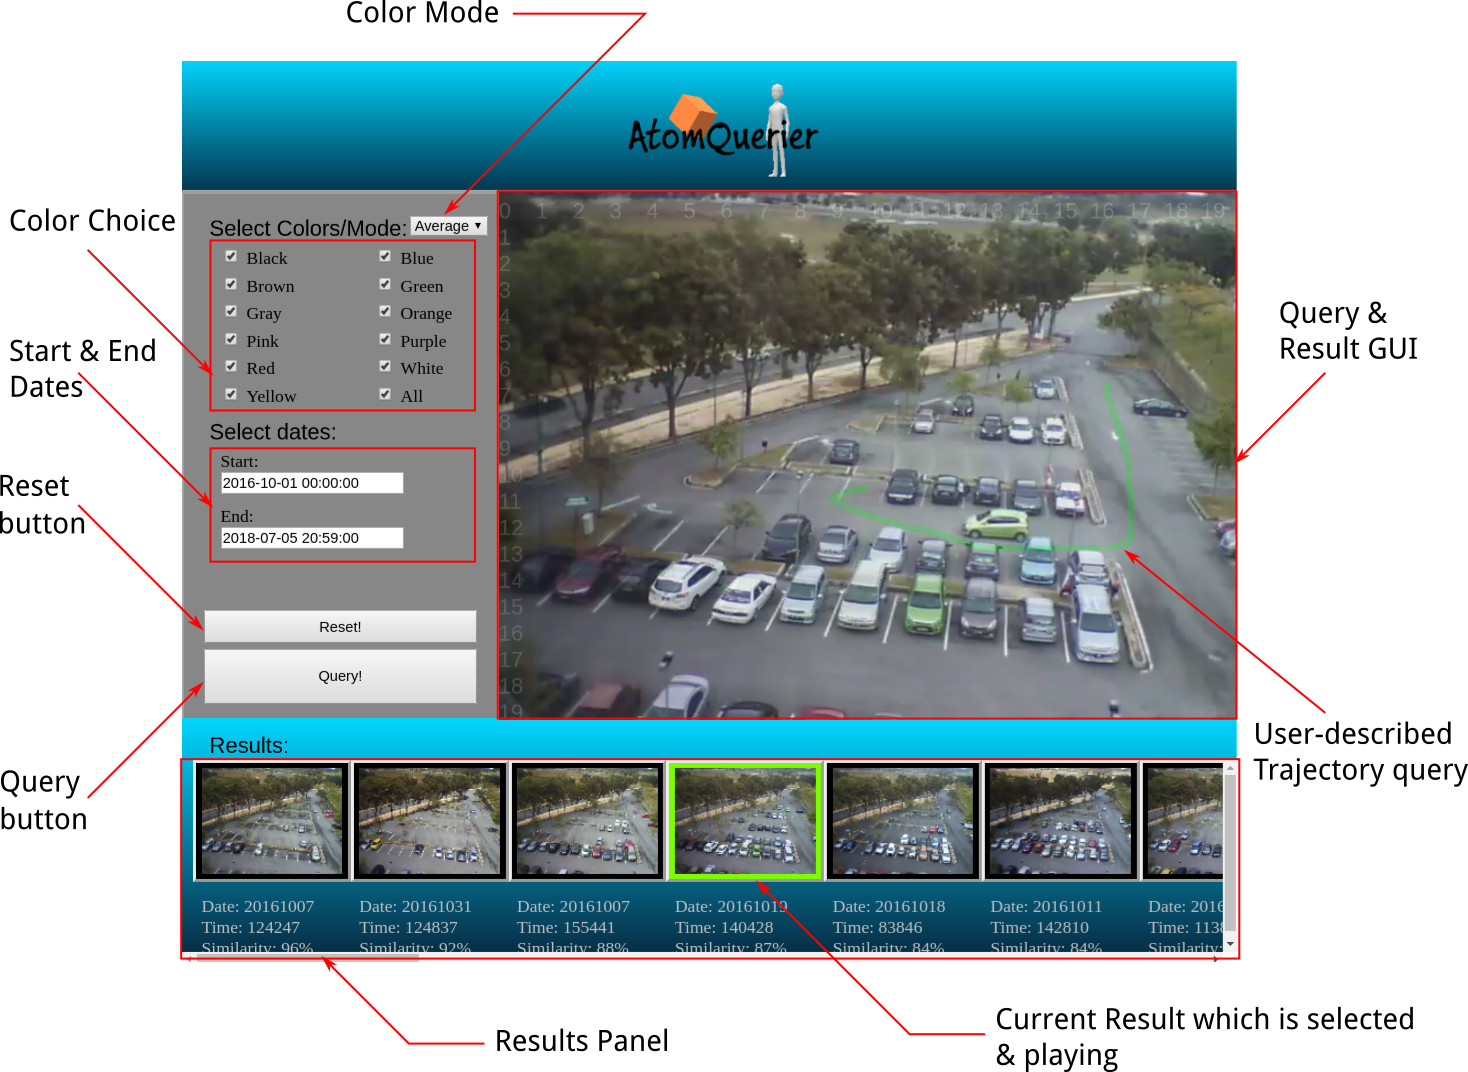
\includegraphics[width=\textwidth]{image/retrievalTwo/VISERinterface2.png}
\caption{Search Interface for \versionTwoRet}
\label{fig:versionTwoInterface}
\end{figure}

\subsection{Metrics, Scoring System and Experimental Methodology}
\label{sec:retrieval-metrics}
The following sub-sections describe the scoring system, metrics as well as the evaluation process of the proposed method described in Section \ref{section:versionTwo}. With the main objective of providing users with results that closely resemble the given query, results which have a higher relevancy are ranked higher in the retrieved result list. In this setting, the performance of the proposed method is measured using two feasible metrics: \textit{Precision@K} and normalised Discounted Cumulative Gain (\textit{nDCG}).

The \textit{Precision@K} metric is used to identify the number of retrieved results which are relevant to the user while the \textit{nDCG} metrics is used to measure how well the retrieval engine's results were ranked or sorted for the end
users. The intuition behind the classic Discounted Cumulative Gain (\textit{DCG}) metric~\cite{jarvelin2002cumulated} is that highly relevant results are more useful when it appears higher in rank (hence, a higher gain). This has practical implications; users would not need to go through a large set of results before finding suitable and/or relevant results that the user desires. Likewise, relevant documents which appear lower in the rank should be penalised, hence warranting a discount in its gain.

In order to distinctly evaluate the performance of the proposed method, the evaluation of both the trajectory and colour terms are separated. The separation of both evaluations allow further understanding on how to improve the retrieval engine on various aspects. FOr further practicality, the evaluation methodology proposes to capture the \emph{relevancy} of the retrieval process through a \emph{user-centric} approach. First, a group of volunteers (\emph{i.e.} the users) are introduced to the retrieval engine along with its features and how the interface system works. A few sample use cases were demonstrated to the volunteers. Next, the volunteers were given full control over the user interface and were allowed to draw any query that they were interested in. They were then tasked to provide feedback by rating each result on a scale of 1 to 5, with 5 being a result that most closely resembles the input query and vice versa.

The volunteers are given full control to draw the input query $\mathbb{P}$ as to mimic a real world scenario. The volunteers were advised to draw realistic looking trajectories that are mainly on the road areas. As there are no limitations on what could be drawn on the search canvas, it was not feasible to  obtain the ``ground-truth'' annotation for every possible motion within the chosen one month's worth of data. Hence, the recall rate could not be viably measured for this retrieval engine. While \textit{Precision@K} metrics is a commonly used metric in retrieval systems, the main disadvantage of this metric is that the evaluation process is done in a rather coarse manner. This is because it only provides a binary evaluation of whether or not a particular result is relevant to the query. On the other hand, the \textit{DCG} metric is able to provide a more granular evaluation of the proposed method as the results are evaluated based on its ordered relevancy rank. Figure~\ref{fig:dcgGain} illustrates the decreasing gain value of each result as the ranking of the
result increases.
\begin{figure}[!tb]
\centering
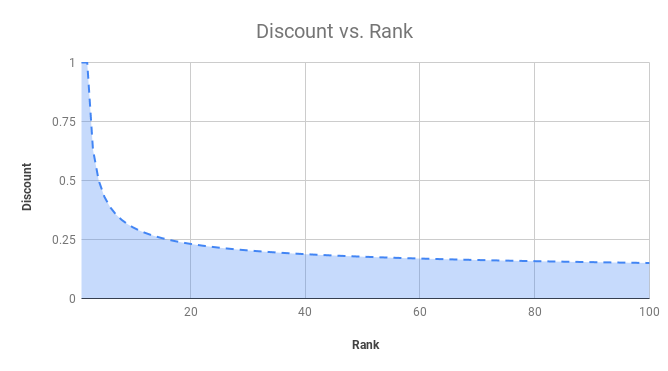
\includegraphics[width=0.9\textwidth]{image/retrievalTwo/discountvsrank.png}
\caption{The Discounted Gain Decreases Exponentially as Rank Increases}
\label{fig:dcgGain}       % Give a unique label
\end{figure}
\begin{equation}
\label{eq:DCGk}
DCG_p = \sum_{p=1}^k\frac{REL_{p}}{\log_2 (\max (p,2))}
\end{equation}
% $DCG@K = \sum_{i=i}^K\frac{REL_{i}}{\log_2 (\max (i,2))}$

Since the Discounted Cumulative Gain metric shown in Equation~\ref{eq:DCGk} produces an unbounded value ([0, $\infty$) range), it is not suitable for use when averaging across multiple independent queries. In order to make use of the \textit{DCG} metric, the normalized version (\textit{nDCG}) shown in Equation~\ref{eq:nDCG} where
the values are now bounded within a [0, 1] range is used instead.
\begin{align}
\label{eq:nDCG}
\textit{nDCG}_k = \frac{DCG_k}{IDCG_k}
\end{align}
$IDCG_P$ is the ideal $DCG$ score at Rank $k$ in the ideal ranking order.

The following subsections provides in-depth details of the experimental methodology that is designed for the evaluation of the retrieval engine's ability to retrieve both the vehicle trajectory and colours.

\subsubsection{Vehicle Trajectory}
The volunteers are given full control of the user interface and are tasked to draw at least 1 trajectory as input query. Upon obtaining results from the query, they were then asked to rate each of the resulting trajectory video shot on a discrete scale from 1 to 5, where 1 signifies the least relevant and 5 being the most relevant.

Each query would return a maximum of 25 randomly ordered results. This was done intentionally to remove any preconceived idea of how the results may have been ordered, which would affect the way the retrieved results are judged. By removing the bias, the volunteers are more likely to provide a fair and sound evaluation for each result set, hence increasing the credibility of the overall results.

\subsubsection{Vehicle colour \& colour mode}
\label{subsec:vehColor}
For the evaluation of the vehicle colours, a list of 330 video snippets (30 video snippets for each of the 11 common colours) were presented to the volunteers. These video snippets were selected using the top 30 results in the database which contained the highest probability score for each of the 11
colours. The volunteers were then asked to determine the relevance of the colour term to that particular vehicle for each of the 330 video snippets on the similar discrete scale of 1 to 5.

To comprehensively evaluate the performance of the colour semantic extraction process which was introduced in Section \ref{section:versiontwoColor}, three other colour modes were included in the evaluation process. These colour modes represent variations of how the colour terms were extracted based on different colour spaces and distance metrics. These variations are listed in Table \ref{table:ColorVariation}.
\begin{table}[tb!]\centering
\begin{tabular}{|c|l|}
\hline
Colour & Distance Metrics \\
Mode &  \\
\hline
LUV &
\begin{tabular}{lcl}
\\
\small
$\mean{r}$ &  $=$  & $\frac{C_{1R} + C_{2R}}{2}$\\
$\Delta R$ & $=$ & $C_{1R} - C_{2R}$\\
$\Delta G$ & $=$ & $C_{1G} - C_{2G}$\\
$\Delta B$ & $=$ & $C_{1B} - C_{2B}$\\
\\
$\Delta Colour_{LUV}$ & $=$ &$\sqrt{(2 + \frac{\mean{r}}{256}) \times \Delta R^{2} + 4 \times \Delta G^{2} + (2 + \frac{255 - \mean{r}}{256}) \times \Delta B^{2}}$
\\
\hspace{4em}& & \\
\end{tabular}\\
\hline
HSV &
\begin{tabular}{lcl}
\\
% \multicolumn{3}{c}{(As introduced in Section \ref{section:versionOneColorExtract})}
\\

$\Delta{H}$ & $=$ & $\min\{ \mid H_{GT} - H \mid,  180^{\circ} - \mid H_{GT} - H \mid  \}$ \\
$\Delta{S}$ & $=$ & $S_{GT} - S$ \\
$\Delta{V}$ &  $=$ & $V_{GT} - V$ \\
\\
$\Delta Colour_{HSV}$ & $=$ & $\sqrt{\Delta{H}^{2} + \Delta{S}^{2}  + \Delta{V}^{2} }$
\\
\hspace{4em}& & \\
\end{tabular}\\
\hline
Lab &
\begin{tabular}{lcl}
\\
$\Delta L$ & $=$ & $C_{1L} - C_{2L}$\\
$\Delta a$ & $=$ & $C_{1a} - C_{2a}$\\
$\Delta b$ & $=$ & $C_{1b} - C_{2b}$\\
\\
$\Delta{Colour_{Lab}}$ & $=$ & $\sqrt{\Delta{L}^{2} + \Delta{a}^{2}  + \Delta{b}^{2} }$
\\
\hspace{5em}& & \\
\end{tabular}\\
\hline
Average &
\begin{tabular}{lcl}
\\
$\Delta{Colour_{Average}}$ & $=$ & $\frac{\Delta{Colour_{LUV}} + \Delta{Colour_{HSV}} + \Delta{Colour_{Lab}}}{3}$
\\
\hspace{4em}& & \\
\end{tabular}\\
\hline
\end{tabular}
  \caption{Formulation of Different COlour Distance Modes Used}
\label{table:ColorVariation}
\end{table}

\subsection{Results and Analysis}

The results for both evaluations (Vehicle Trajectory \& Vehicle Colour) are reported in this section. As the results were evaluated on a discrete scale from 1 to 5, the results are first converted into a binary evaluation (True (1) /
False (0)) for the purpose of \textit{Precision@K} metric. For ease of computation, results scoring with an average of 3 and above are considered as relevant to the query. The $n$-th relevant results (\emph{i.e.} True (1)) from among all $K$ recalled results contribute to the
\textit{Precision@K} score set out in Equation \ref{eq:p@k}):
\begin{equation}
\label{eq:p@k}
Precision@K =  \frac{\sum_{n=1}^K \delta}{K}
\end{equation}
where 
\begin{equation}
\delta=1, \qquad \text{if} \frac{1}{\Psi}\sum S_{n,\psi} \geq 3
\end{equation}
The overall score for the $n$-th result is averaged over the score decisions $S_{n,\psi}$ made by $\Psi$ number of volunteers.

\subsubsection{Vehicle Trajectory}
A total of eleven restriction-free trajectories were drawn by six volunteers. The volunteers were allowed to draw any kind of desired trajectory on the input canvas. Figure \ref{fig:versionTwoTrajquery} shows a compilation of these trajectories overlaid over the car park scene, these trajectories covered a majority of those typically found in the recorded scene while showing a good mixture of different query variations and lengths. Even though some of the queries exceeded the tracking area of the tracker, the retrieval engine still managed to retrieved results with the closest resemblance to the given queries. As previously mentioned, the performance of the retrieval engine was measured using \textit{Precision@K} along with the \textit{normalised Discounted Cumulative Gain} (\textit{nDCG}) metric.
\begin{figure}[!t]
  \centering
    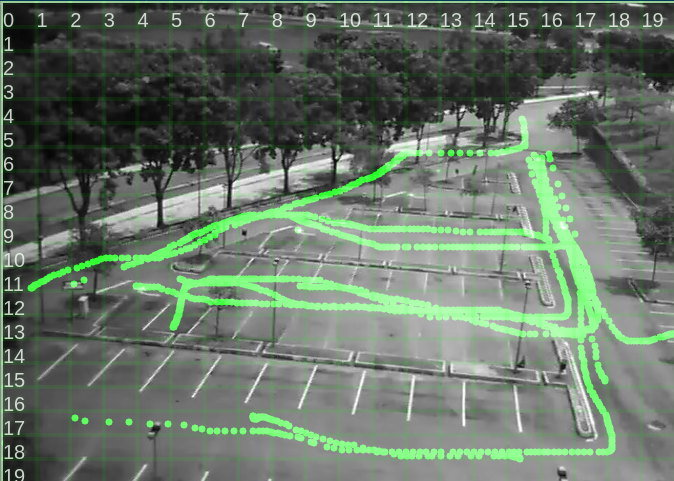
\includegraphics[width=0.8\linewidth]{image/retrievalTwo/trajquery.png}
  \caption{Compilation of Trajectory Queries Provided by Volunteers}
  \label{fig:versionTwoTrajquery}
\end{figure}
\begin{figure}[!t]
  \centering
    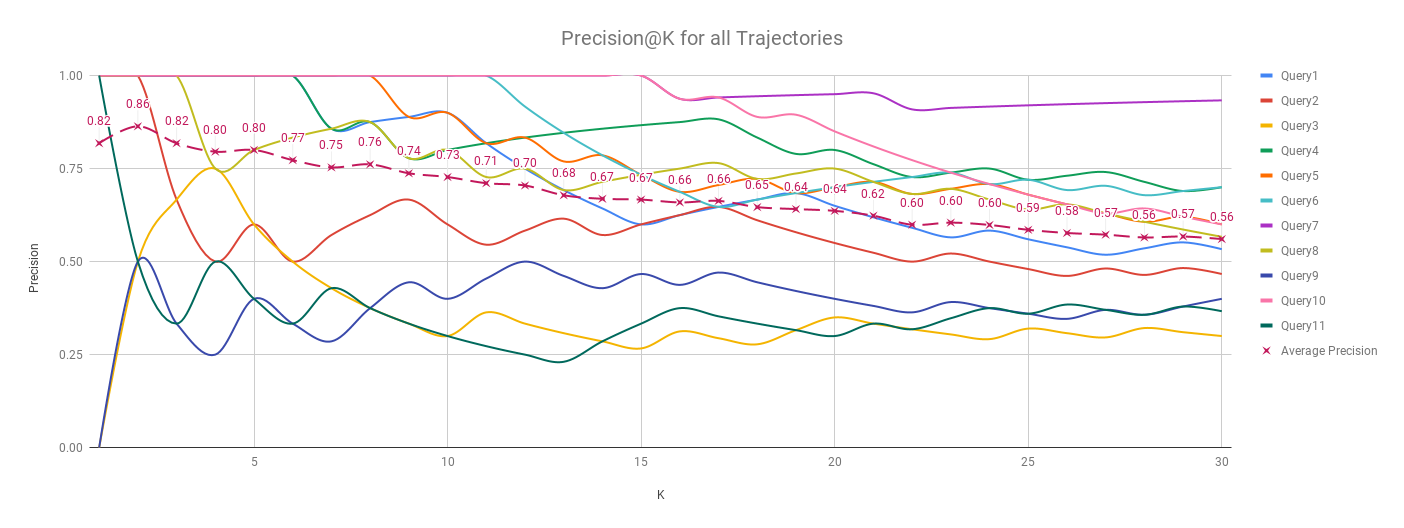
\includegraphics[width=\linewidth]{image/retrievalTwo/p@k.png}
  \caption{Precision@K for All Evaluated Trajectory Queries}
  \label{fig:versionTwoPreAtK}
\end{figure}

Even though the errors from the selected tracker~\cite{lim2017} did affect the retrieval process to a small extent, results that were obviously impacted by tracker error were not removed to provide a realistic view of the retrieval engine's performance when working with off-the-shelf trackers which are widely available. First, the \textit{Precision@K} of the retrieval engine was measured and shown in Figure \ref{fig:versionTwoPreAtK} where the average across all results were also plotted (in dashed line). The result shows that the retrieval engine is reasonably successful in retrieving video shots which were relevant to the users' queries with an average precision of 76\% with a steady decline in its precision as the $K$ (number of results) increases. This was an expected outcome as it is a common occurrence in typical retrieval systems.

Next, in order to determine the retrieval engine's overall performance in regards to how the results were ordered, the average \textit{nDCG} score for all eleven trajectory queries were measured and plotted in Figure~\ref{fig:ndcgWithError}. On the whole, the average \textit{nDCG} score hovers around the 83\% region, which literally indicates that the results were ranked in the best possible manner 83\% of the time. In an ideal scenario, the scores would return 1 (or 100\%), signifying that the results were ranked perfectly. In this experiment, the \textit{nDCG} score shows an increase when the number of retrieved results increases. %While this is not desirable, this behaviour was expected in a non-ideal
condition.
\begin{figure}[!tb]
  \centering
    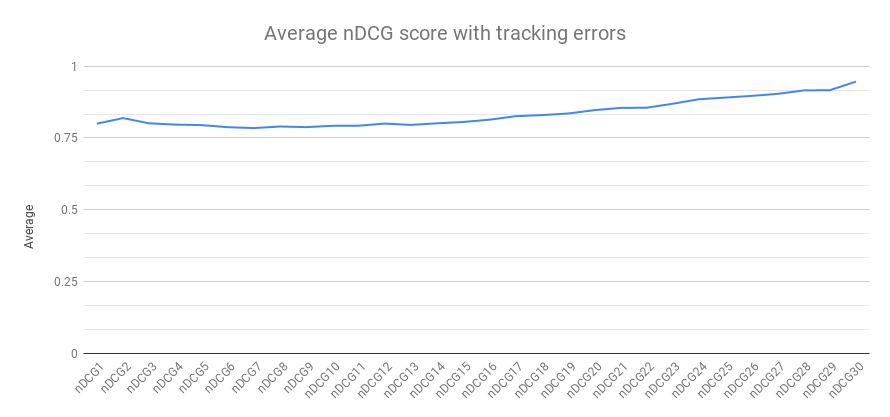
\includegraphics[width=0.9\linewidth]{image/retrievalTwo/averageNDCG.png}
  \caption{Average Normalised Discounted Cumulative Gain Score}
  \label{fig:ndcgWithError}
\end{figure}

To further break down the evaluation process of the retrieval engine's performance (in similar fashion to the previous retrieval model's evaluation), the trajectory queries were also divided into two categories: \textit{simple} and \textit{complex} trajectories. To reiterate, \textit{simple} trajectories refer to trajectories that moves in a single direction without any turning (such as a straight line) while \textit{complex} trajectories refer to movements which consist of more than one simple motion, \emph{e.g.} a turn into a junction, a U-turn, or multiple turns. Table \ref{table:versionTwoComplexSimple} shows the category of each query while the \textit{Precision@K} results are plotted in Figure~\ref{fig:versionTwoPatKAll}.

For simple trajectories, the Precision@K scores a high 100\% at the beginning and slowly decreases to around 68\% as the number of retrieved results ($K$) increases. All the simple queries showed rather consistent results, which are as expected. As for complex trajectories, the precision at $K=1$ started at 67\% and it dropped further to 46\% at the end of 30 ($K=30$) results. Even though Query 1 and Query 6 belong to the complex trajectory category, the first 10 results shows rather high precision scores. However, the majority of the other complex trajectories did not perform as well as Query 1 and Query 6. The overall \textit{Precision@K} results show an expected behaviour where the precision would be high in the early $K$ values, and would slowly decrease as $K$ increases.
% Please add the following required packages to your document preamble:
% \usepackage{multirow}
\begin{table}[!tb] \centering
\begin{tabular}{|c|c|c|}
\hline
\multicolumn{1}{|c|}{\textbf{Trajectory Category}} & \textbf{Query Number} & \textbf{Minimap}\\ \hline
\multirow{5}{*}{Simple} & Query 4 & 
\includegraphics{image/minimaps/query_04.png} \\ \cline{2-3}
 & Query 5 & 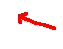
\includegraphics{image/minimaps/query_05.png} \\ \cline{2-3}
 & Query 7 & 
\includegraphics{image/minimaps/query_07.png} \\ \cline{2-3}
 & Query 8 & 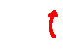
\includegraphics{image/minimaps/query_08.png} \\ \cline{2-3}
 & Query 10 & 
\includegraphics{image/minimaps/query_10.png} \\ \hline
\multirow{6}{*}{Complex} & Query 1 & 
\includegraphics{image/minimaps/query_01.png} \\ \cline{2-3}
 & Query 2 & 
\includegraphics{image/minimaps/query_02.png} \\ \cline{2-3}
 & Query 3 & 
\includegraphics{image/minimaps/query_03.png} \\ \cline{2-3}
 & Query 6 & 
\includegraphics{image/minimaps/query_06.png} \\ \cline{2-3}
 & Query 9 & 
\includegraphics{image/minimaps/query_09.png} \\ \cline{2-3}
 & Query 11 & 
\includegraphics{image/minimaps/query_11.png} \\ \hline
\end{tabular}
\caption{Queries, Minimaps and the Corresponding Trajectory Type}
\label{table:versionTwoComplexSimple}
\end{table}
On a whole, when taken together, all queries showed reasonably good performances in terms of the precision score. However, when evaluated individually, the \textit{complex} queries showed significantly poorer results. 

The \textit{nDCG} scores for both \textit{simple} and \textit{complex} trajectory queries were evaluated and plotted in Figure~\ref{fig:versionTwoNDCG}(a) and Figure \ref{fig:versionTwoNDCG}(b) respectively. Contrary to the coarser results with \textit{Precision@K}, the \textit{nDCG} score is able to provide an in-depth evaluation as it takes the relevancy of ranking into consideration.
\begin{figure}[tb!]
  \centering
\begin{tabular}{c}
 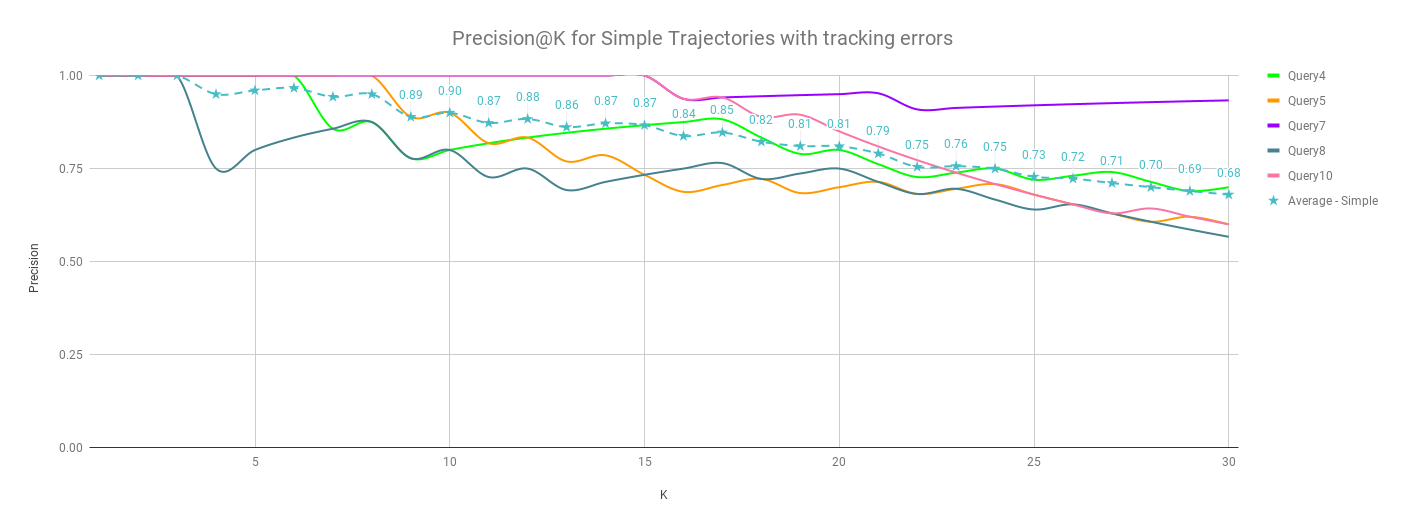
\includegraphics[width=0.9\linewidth]{image/retrievalTwo/p@k_simple.png}\\
 (a) \textit{Precision@K} for Simple Trajectories \\
 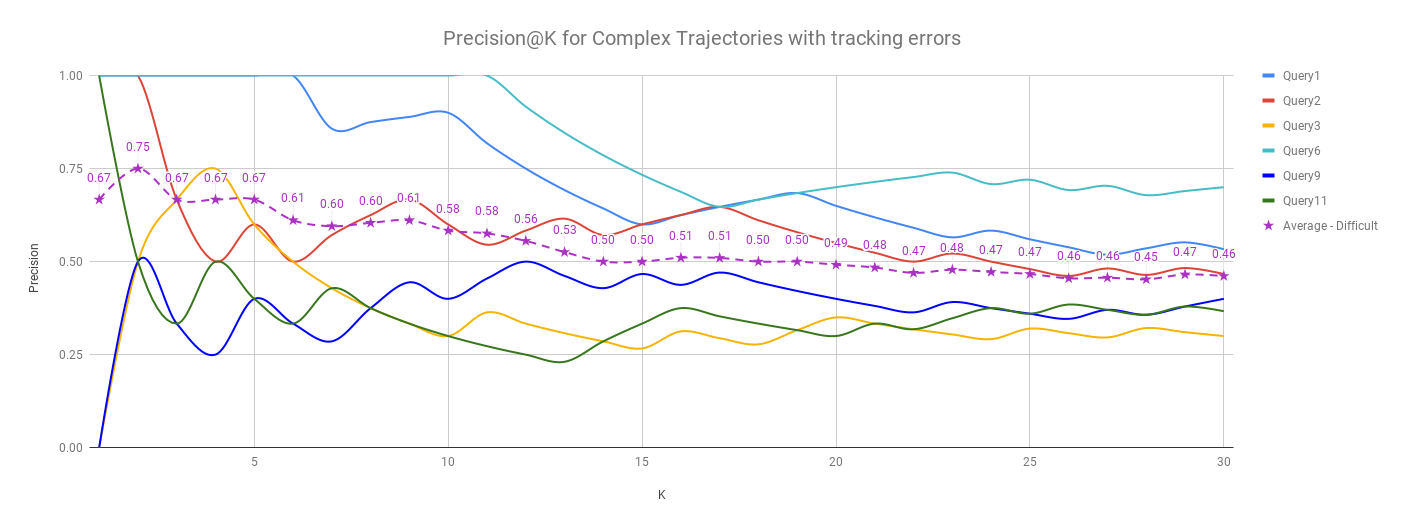
\includegraphics[width=0.9\linewidth]{image/retrievalTwo/p@k_complex.png} \\
 (b) \textit{Precision@K} for Complex Trajectories
\end{tabular}
\caption{\textit{Precision@K} for Simple and Complex Trajectories Queries}
\label{fig:versionTwoPatKAll}
\end{figure}
\begin{figure}[tb!]
  \centering
  \begin{tabular}{c}
   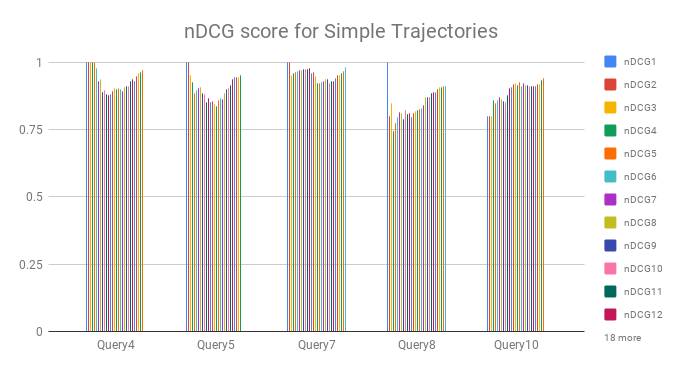
\includegraphics[width=0.9\linewidth]{image/retrievalTwo/ndcgSimple.png}\\
   (a) \textit{nDCG} for Simple Trajectories \\
   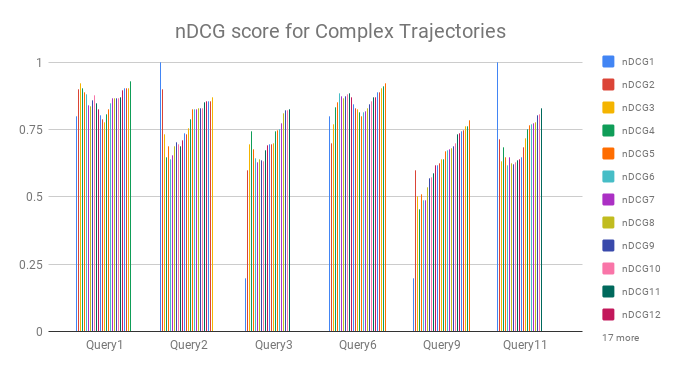
\includegraphics[width=0.9\linewidth]{image/retrievalTwo/ndcgComplex.png} \\
   (b) \textit{nDCG} for Complex Trajectories
  \end{tabular}
  \caption{Normalised Discounted Cumulative Gain for Simple and Complex
  Trajectories Queries}
  \label{fig:versionTwoNDCG}
\end{figure}

Based on the graph, the difference between the simple and complex trajectories are rather distinct. The overall $nDCG$ scores for the queries of simple trajectories hover high around the 91\% region while the $nDCG$ scores for complex trajectories are around the 75\% level on average. The results here show that the retrieval engine was able to sort simple trajectories according to the order of relevancy while it encountered some difficulty organising the complex trajectories using the $D_{chamfer}$ distance measure.

Additional comparisons between the Chamfer Distance and various other distance measures were also performed to further understand the differences, advantages and properties of these methods. Table~\ref{table:DistanceCompare} presents a compilation of 7 different test cases on a single sample ground truth data. These test cases were then tested using 5 different distance measures: Chamfer Distance, Dynamic Time Warping, Hausdorff Distance, Earth Mover Distance, and Euclidean Distance. In all cases, smaller numbers would represent smaller distances (corresponding to higher similarities) while larger numbers represent larger distances (or lower similarities).

As a baseline comparison, a simplistic approach using Euclidean Distance was also considered. The results obtained from Euclidean Distance showed minimal difference in the raw results when comparing between the best- and worst-performing test cases. %While the normalised results showed better results, the normalised result is not a useful metrics as it only represents the distribution in the 7 test cases. 
In an actual retrieval process, we were not able to obtain these scores during runtime. Based on the results in Table \ref{table:DistanceCompare}, it is noticeable that the Earth Mover Distance (EMD) favours similar shapes as it is able to effectively deal with slight shape variations among the retrieved trajectories. While this may be useful in other applications that are not order-sensitive, this is not a desirable property in the context of retrieving motions from a car park setting. As expected, the EMD measure is heavily penalised in Test 1, which contains a mirrored shape.

In the case of Hausdorff distance, it can be observed that this distance measure often measures the maximum distance of a set to the nearest point in the other set which is commonly used for matching sets of images. It is also observed that this distance measure was not able to handle Test 2 which contains directional inputs, this shows that this metric is also a less suitable candidate for our retrieval engine. The overall results shows that both Chamfer Distance and Dynamic Time Warping were good candidate methods as they have relatively good and similar performances in all 7 test cases. However, the Chamfer Distance was able to return a higher difference ratio between the best- and worst-performing test cases. This attribute is desirable and would be very useful for ranking a large number of trajectories from the database.

Even though the overall results using Chamfer Distance were relatively good, the characteristics of this distance measure has its limitations. A close examination of some of the retrieved results as shown in Figure~\ref{fig:chamferDisadvantage}, showed that the Chamfer Distance performed poorly when (i) a trajectory is compared against a much shorter trajectory that intersects closely at a particular point or segment, or (ii) two trajectories of similar shape turning into 2 different junctions. In both examples, the obtained $D_{chamfer}$ values were relatively low, hence these results could potentially be retrieved at a high rank.
\begin{figure}[tb!]
  \centering
\begin{tabular}{cc }
 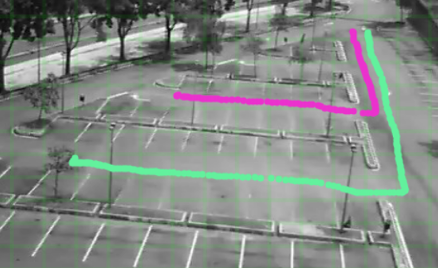
\includegraphics[width=0.47\linewidth]{image/retrievalTwo/chamferDisadv2.png} &
 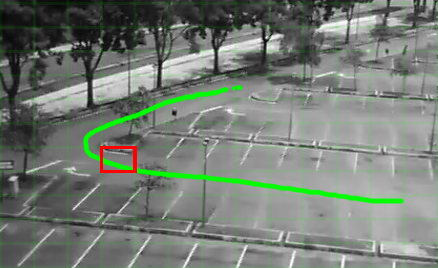
\includegraphics[width=0.47\linewidth]{image/retrievalTwo/chamferDisadv1.png} \\
 (a) Two trajectories with similar shape &
 (b) Trajectory intersecting with a point \\
\end{tabular}
\caption{Disadvantages of Chamfer Distance} \label{fig:chamferDisadvantage}
\end{figure}

% Please add the following required packages to your document preamble:
% \usepackage{graphicx}
% \usepackage{lscape}
\begin{landscape}

\begin{table}[]
\resizebox{23cm}{!}{%
\centering
\begin{tabular}{|l||l|l|l|l|l|l|l|}
\hline
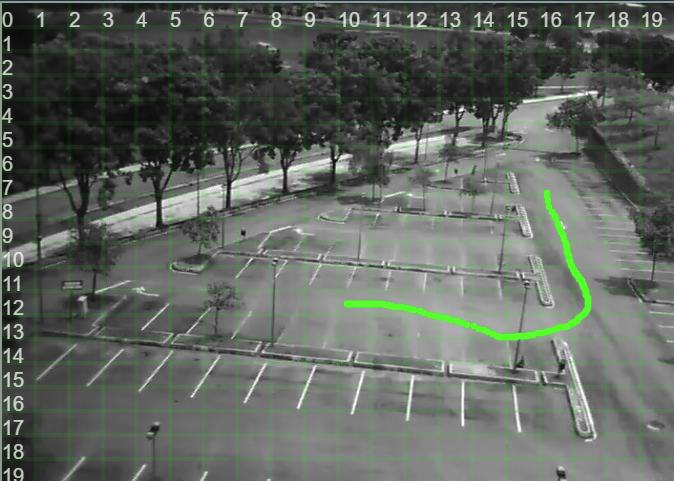
\includegraphics[scale=0.25]{image/suppResults/gt.PNG}
 & 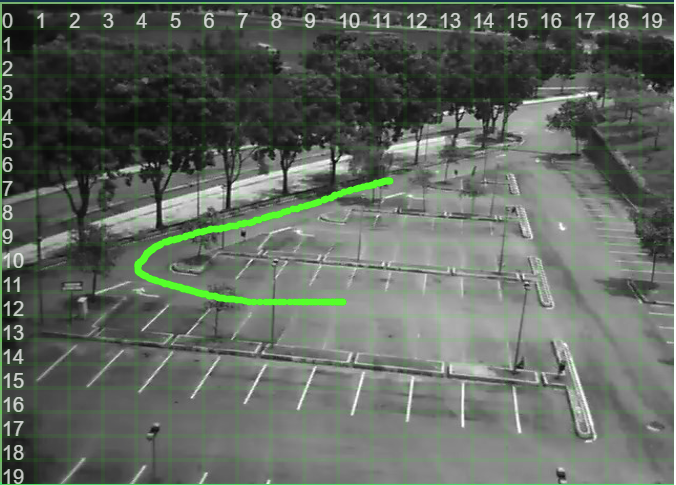
\includegraphics[scale=0.25]{image/suppResults/q1.PNG}
 & 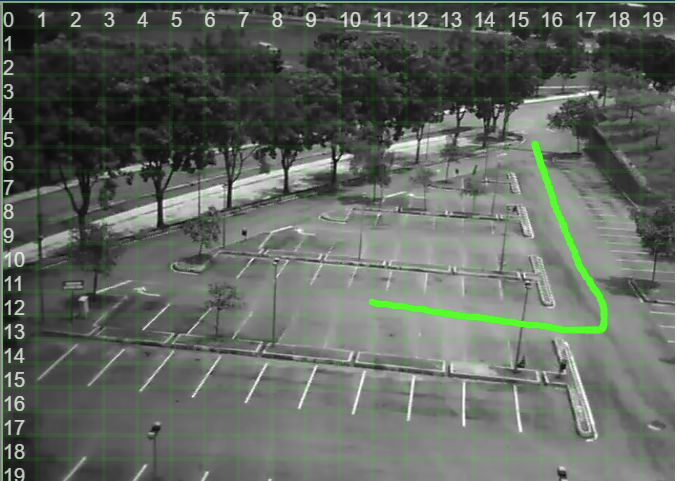
\includegraphics[scale=0.25]{image/suppResults/q2.PNG}
 & 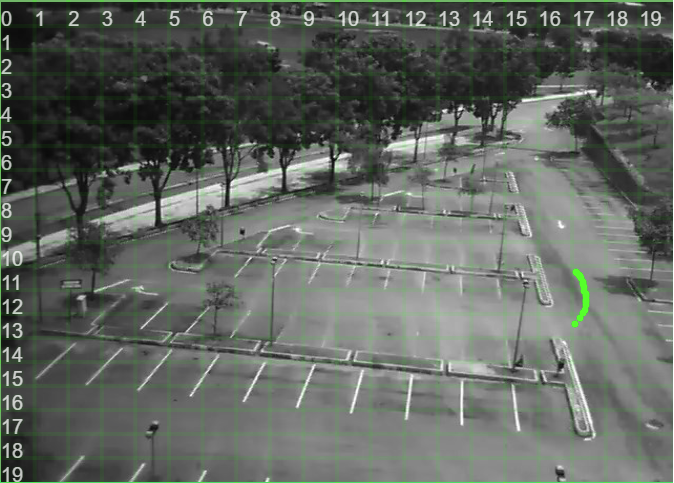
\includegraphics[scale=0.25]{image/suppResults/q3.PNG}
 & 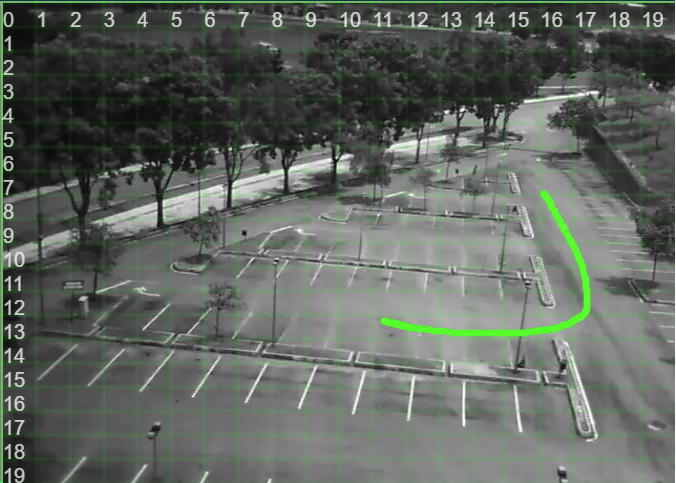
\includegraphics[scale=0.25]{image/suppResults/q4.PNG}
 & 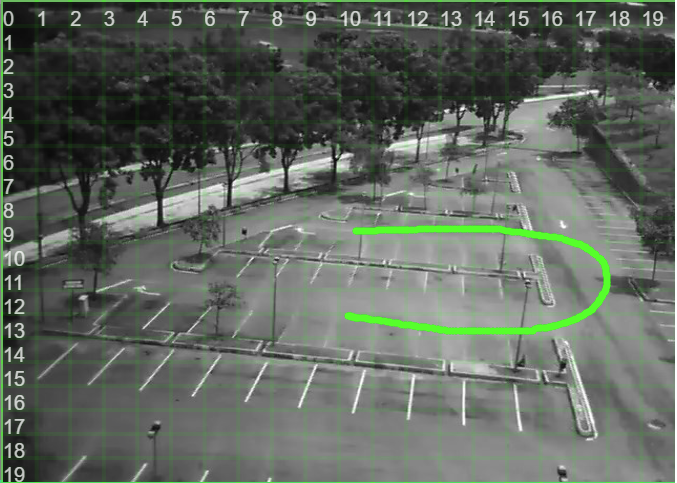
\includegraphics[scale=0.25]{image/suppResults/q5.PNG}
 & 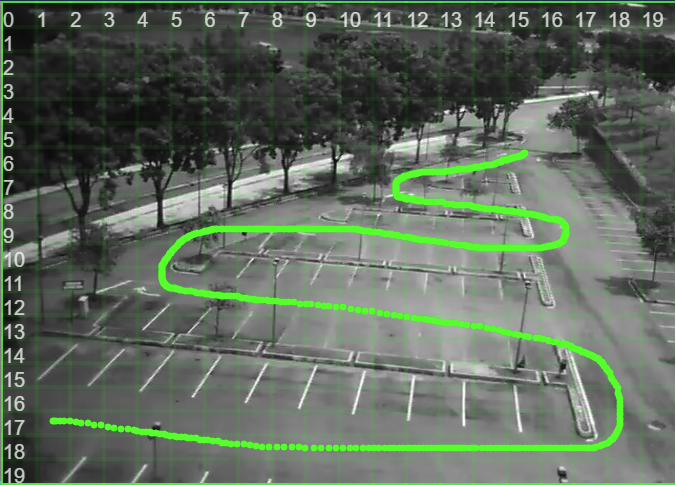
\includegraphics[scale=0.25]{image/suppResults/q6.PNG}
 & 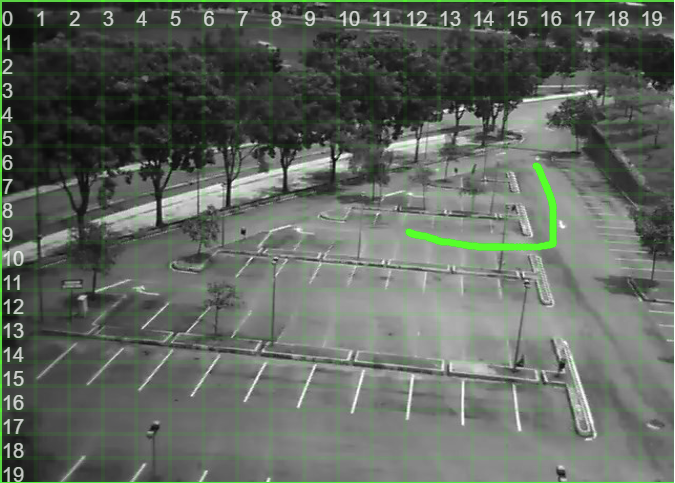
\includegraphics[scale=0.25]{image/suppResults/q7.PNG} \\ \hline
GT Sample & \begin{tabular}[r]{@{}l@{}}Test 1:\\ Mirror\end{tabular} & \begin{tabular}[r]{@{}l@{}}Test 2:\\ Opposite Direction\end{tabular} & \begin{tabular}[r]{@{}l@{}}Test 3:\\ Short Trajectory\end{tabular} & \begin{tabular}[r]{@{}l@{}}Test 4:\\ Highly Resemble GT\end{tabular} & \begin{tabular}[r]{@{}l@{}}Test 5:\\ Partially Resemble GT\end{tabular} & \begin{tabular}[r]{@{}l@{}}Test 6:\\ Long Trajectories\end{tabular} & \begin{tabular}[r]{@{}l@{}}Test 7:\\ Similar Shape\end{tabular} \\ \hline
\textbf{Chamfer Distance} & 0.02565 (1503.21) & 0.0169 (987.84) & 0.0246 (1444.00) & 0.0001 (6.25) & 0.0060 (353.89) & 0.9205 (53937.33) & 0.0062 (361.00) \\ \hline
\textbf{Dynamic Time Warping} & 0.0503 (176.97) & 0.0344 (121.08) & 0.0604 (212.31) & 0.0033 (11.62) & 0.0239 (83.99) & 0.8079 (2841.17) & 0.0198 (69.57) \\ \hline
\textbf{Hausdorff Distance} & 0.2042 (7.07) & 0.0647 (2.24) & 0.2021 (7.00) & 0.0407 (1.41) & 0.0866 (3.00) & 0.2974 (10.30) & 0.1042 (3.61) \\ \hline
\textbf{Earth Mover Distance} & 0.4112 (0.96) & 0.0942 (0.22) & 0.0342 (0.08) & 0.0021 (0.01) & 0.3127 (0.73) & 0.1456 (0.34) & 0.0000 (0.00) \\ \hline
\textbf{Euclidean Distance} & 0.1171 (5.00) & 0.1656 (7.07) & 0.1424 (6.08) & 0.0703 (3.00) & 0.0661 (2.82) & 0.3645 (15.56) & 0.0740 (3.16) \\ \hline
\end{tabular}%
}
\caption{Comparison of 5 distance measures (Chamfer Distance, Dynamic Time Warping, Hausdorff Distance, Earth Mover Distance, Euclidean Distance) in 7 specific test scenarios -- (1) Mirror, (2) Opposite Direction, (3) Short Trajectory, (4) Highly Resemble GT, (5) Partially Resemble GT, (6) Long Trajectories, (7) Similar Shape, against ground truth sample data. Overall results showed the superiority of Chamfer Distance in normalised distances. The actual distance measures are shown in parentheses. Smaller numbers represent higher similarity and vice versa. %Euclidean distance acts as a simplistic approach towards this problem, and was used as a baseline comparison. The results shows that Earth Mover Distance favoured cases where the shapes were similar (Test 7) and penalised a mirrored shape (Test 1). Hausdorff distance failed to provide good dissimilarity score for test 2 which was used to test the ability to differentiate directions. Overall, Chamfer Distance and Dynamic Time Warping method was able to provide comparable results. However, Chamfer Distance came up top as it is able to provide a larger margin between the best and worst test cases. This property is desirable when comparing huge numbers of trajectories.%
}
\label{table:DistanceCompare}
\end{table}
\end{landscape}

However, despite the little flaws observed of the Chamfer Distance, the implementation of $D_{chamfer}$ in the retrieval engine provided relatively good results (Average \textit{Precision@K} = 76\%) that were ranked in an organised and useful manner (\textit{nDCG} score = 83\%). In my opinion, the use of Chamfer Distance can be extended to other datasets of similar properties.

\subsubsection{Vehicle Colour \& Colour Mode}
\label{subsec:vehiclecolourchamferdistanceexperiment}

As mentioned in Section \ref{subsec:vehColor}, a total of 330 video snippets were extracted from the top 30 results of each colour mode. As four colour modes were tested, the six volunteers were split into groups of three persons and were given two sets of data to evaluate. The results of the average \textit{Precision@K} metric for each of the colour modes were tabulated in Figure \ref{fig:colorspace_score} while Table \ref{tab:avg@k} provides an overview of the results from $K=1$ to $K=30$. Similar to the evaluation process of the vehicle trajectories, the volunteers were asked to determine the relevance of the colour term to that particular vehicle for each of the video snippets on a similar discrete scale of 1 to 5.
\begin{table}[!tb]
	\centering
	\caption{Average Precision @ K for Each Colour Metrics}
	\label{tab:avg@k}
\begin{tabular}{c||c|c|c|c|c|c|c|c|c|c}
K & 1 & 2 & 3 & 4 & 5 & 10 & 15 & 20 & 25 & 30  \\ \hline \hline
\rowcolor{yellow} LUV  & 0.91 & 0.91 & 0.91 & 0.86 & 0.85 & 0.69 & 0.62 & 0.60 & 0.63 & 0.60 \\
Lab  & 0.27 & 0.27 & 0.27 & 0.25 & 0.24 & 0.24 & 0.24 & 0.23 & 0.22 & 0.22 \\
HSV & 0.27 & 0.36 & 0.30 & 0.27 & 0.29 & 0.25 & 0.25 & 0.23 & 0.21 & 0.21 \\
Avg & 0.09 & 0.18 & 0.15 & 0.16 & 0.16 & 0.18 & 0.18 & 0.20 & 0.23 & 0.23 \\
\end{tabular}
\end{table}
\begin{figure}[tb!]
  \centering
\begin{tabular}{cc}
 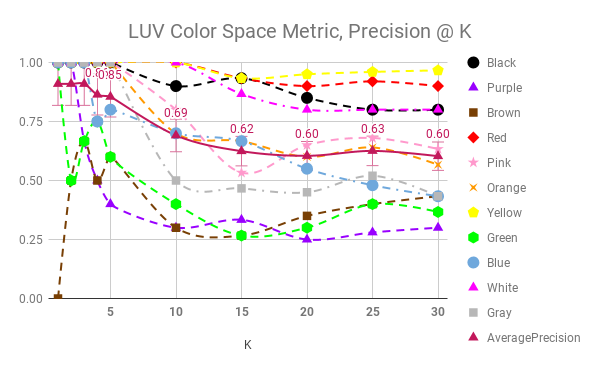
\includegraphics[width=0.5\linewidth]{image/new/luv@k.png} &
 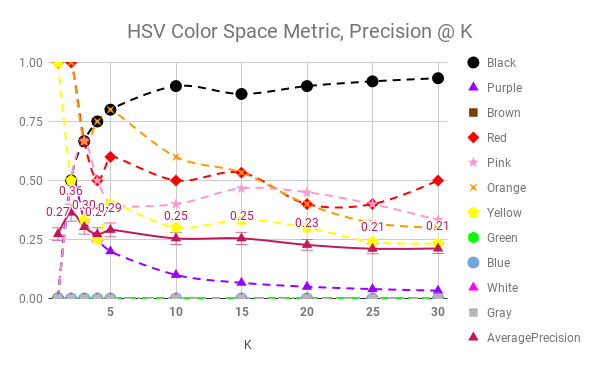
\includegraphics[width=0.5\linewidth]{image/new/hsv@k.png}\\
 (a) LUV colour Mode &
 (b) HSV colour Mode \\
 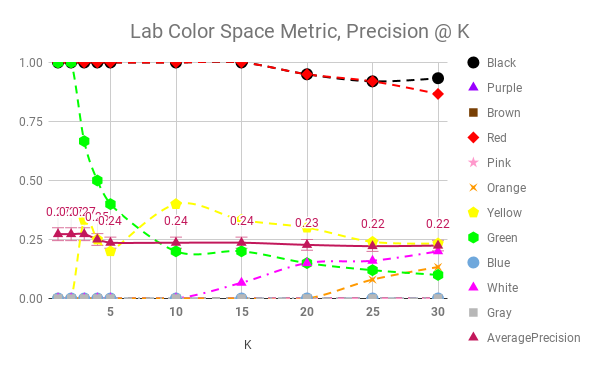
\includegraphics[width=0.5\linewidth]{image/new/lab@k.png} &
 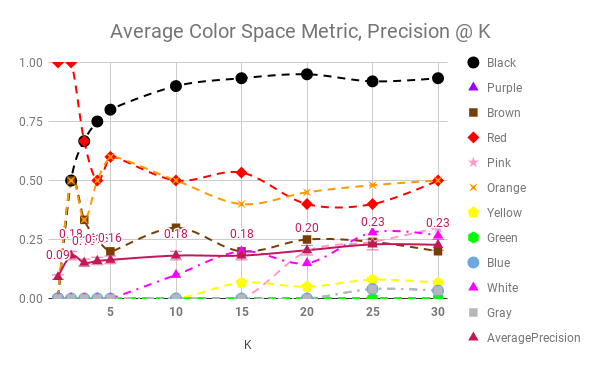
\includegraphics[width=0.5\linewidth]{image/new/avg@k.png} \\
 (c) Lab colour Mode&
 (d) Average colour Mode \\
\end{tabular}
\caption{\textit{Precision@K} for Each Colour Mode}
  \label{fig:colorspace_score}
\end{figure}

Overall, the \textit{Precision@K} results of the LUV colour mode showed the best results among the other colour modes compared. The average precision at $K=1$ is recorded at 91\%, although by $K=10$, the precision has dropped to an average precision of 69\% and then gradually drops to 60\% when $K=30$. The colours `Yellow', `Red', `Black', and `White' showed consistent results throughout the experiment while colours like `Purple', `Green' and `Brown' fared poorly. This is likely because there were not many cars which had highly saturated shades of those colours.

When comparing with other colour modes, `Black' provided relatively consistent results throughout the entire experiment. The average precision for HSV and Lab colour modes staggered at around the 25\% region. It is also observed that the retrieval of `Red' and `Black' colour vehicles is significantly better than other colours when the Lab colour space is used, with the average precision in the vicinity of 90\%.

During the preparation phase of the experimental methodology, the average colour mode was designed with the goal of maximising the strength of each colour mode while averaging out the weaknesses. However, based on the conducted experiment, it was surprising to see the underwhelming performance of the HSV and Lab colour mode, which impacted the average colour mode. %Hence, the average colour mode also took a dive in terms of the precision. 
However, the average colour mode did live up to its expectation in maximising the strengths of each colour modes. Based on the tabulated results, the precision when retrieving `Black' colour vehicles was good except for the initial precision at small $K$ values which were unexpected.

To further analyse the performance of the colour modes used, the confusion matrix of each colour mode is plotted in Figure~\ref{fig:colorspace_Confuscore} using the top 30 results for each colour term %(with a total of 330 results for each colour space).  
The X-axis represents the Actual Colour, while the Y-axis represents the Predicted Colour. The colours in the confusion matrix are arranged in the following order: Black, Purple, Brown, Red, Pink, Orange, Yellow, Green, Blue, White, Gray. This colours are ordered based on its perceived similarity to each other in terms of their saturation and brightness. In the figure, the X-axis also contains an additional last row which indicates the number of results that had tracking errors (from the initial tracking phase); these were excluded from consideration.
\begin{figure}[tb!]
  \centering
  \begin{tabular}{cc}
    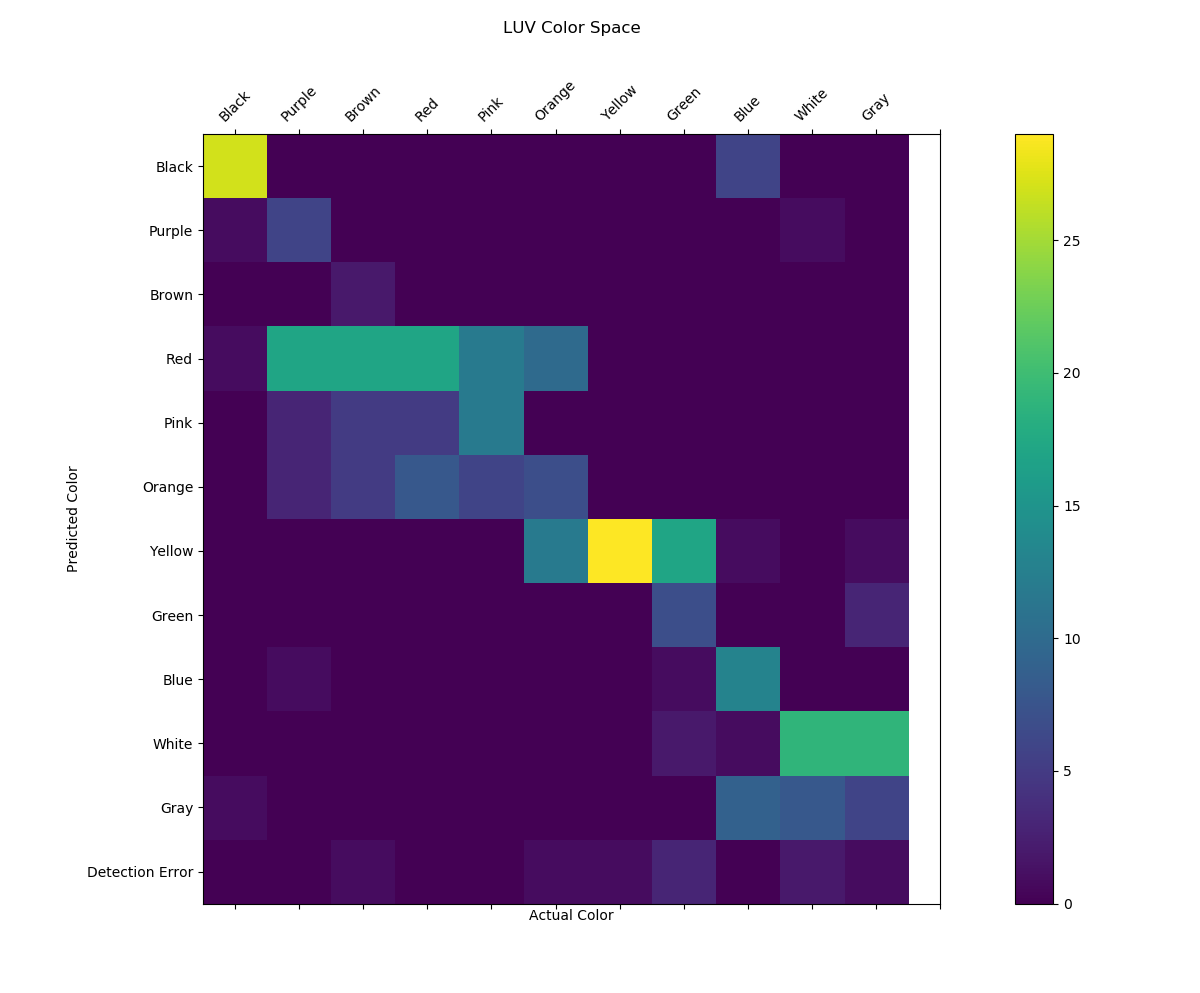
\includegraphics[width=0.4\linewidth]{image/retrievalTwo/luvCM.png} &
    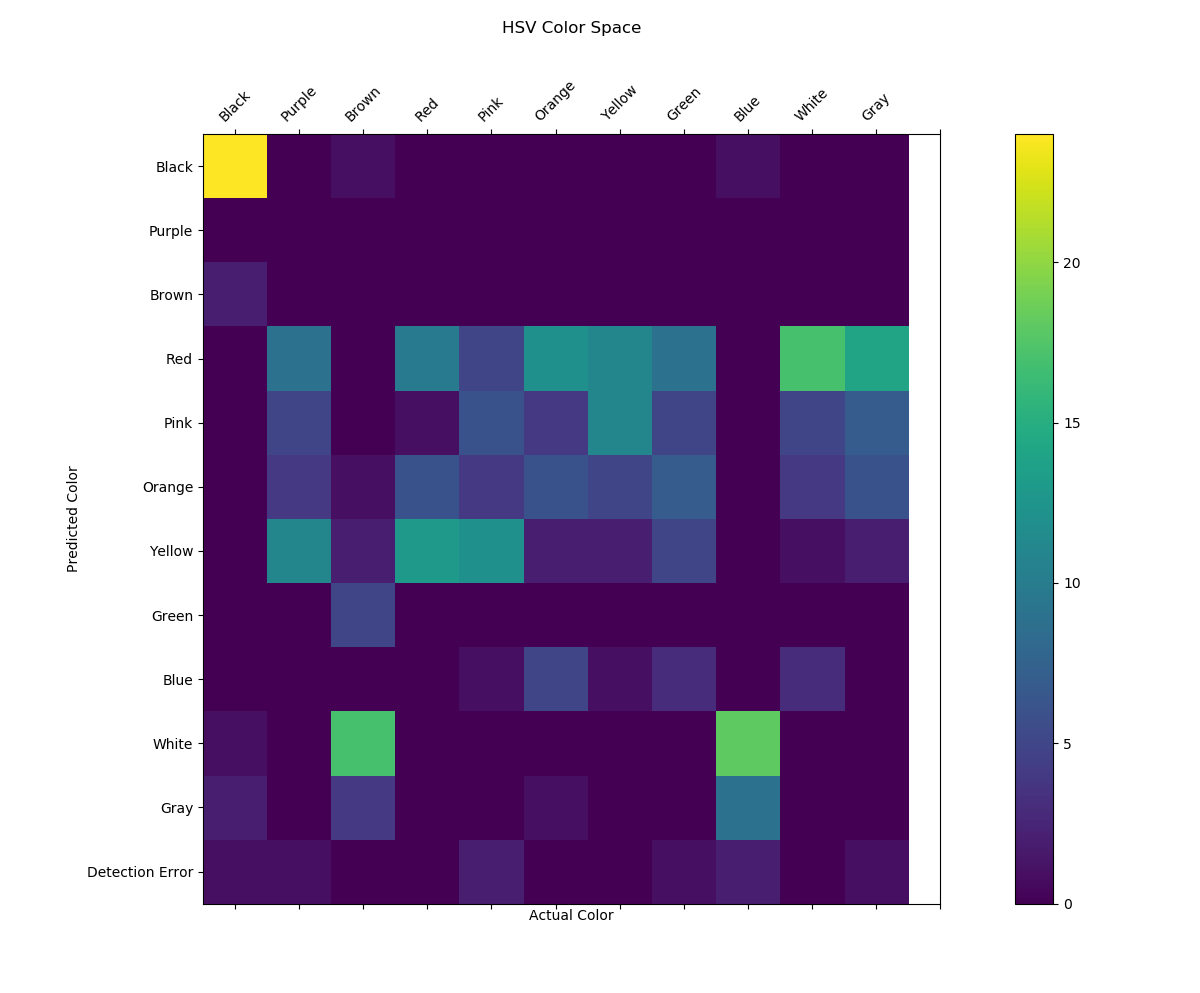
\includegraphics[width=0.4\linewidth]{image/retrievalTwo/hsvCM.png} \\
    (a) LUV colour Mode & (b) HSV colour Mode \\
    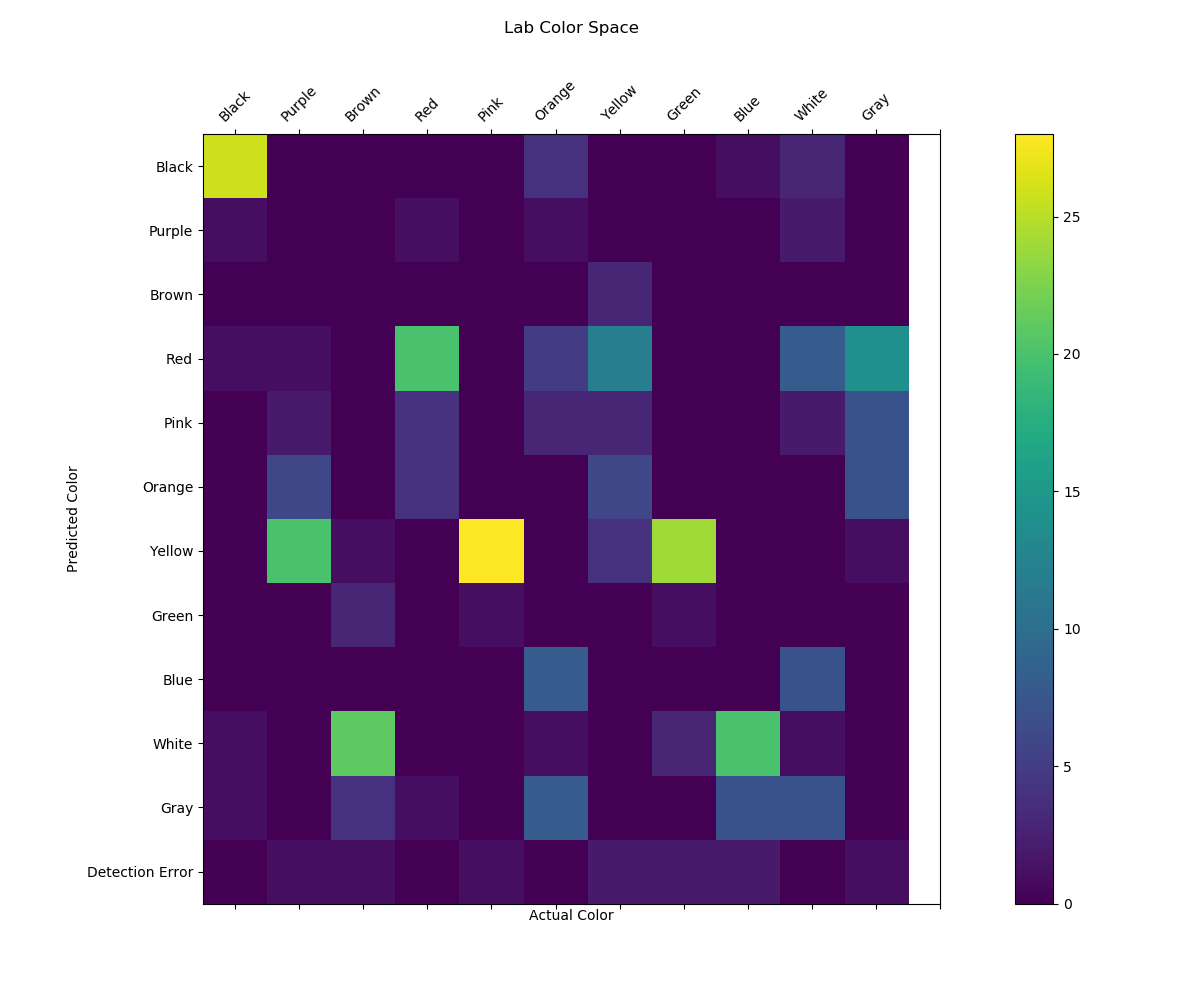
\includegraphics[width=0.4\linewidth]{image/retrievalTwo/labCM.png} &
    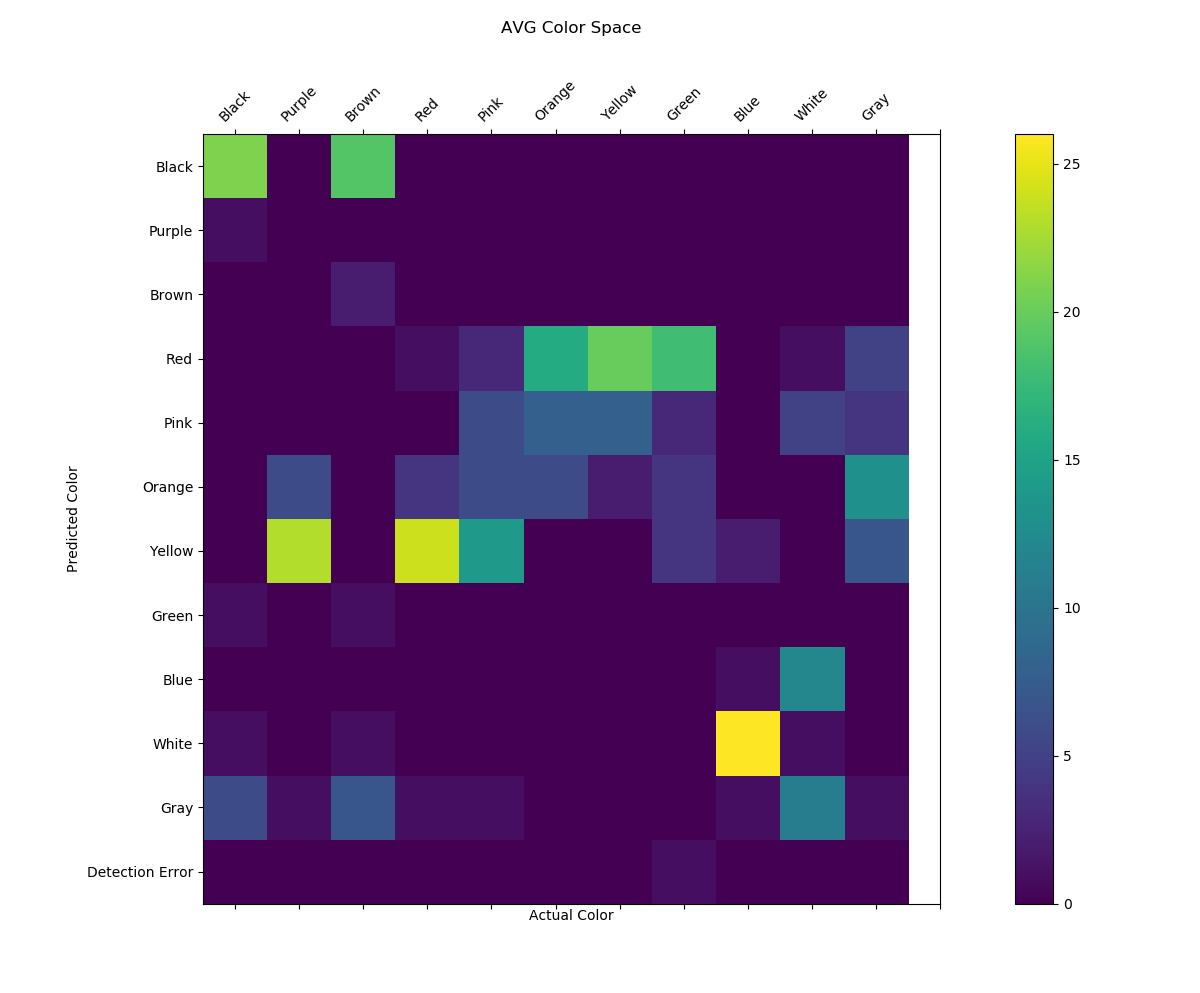
\includegraphics[width=0.4\linewidth]{image/retrievalTwo/avgCM.png} \\
    (c) Lab colour Mode & (d) Average colour Mode \\
  \end{tabular}
  \caption{Comparison Between the colour Modes Using Confusion Matrix}
  \label{fig:colorspace_Confuscore}
\end{figure}

Upon further inspection of the confusion matrices (in Figure \ref{fig:colorspace_Confuscore}), the results show somewhat similar characteristics as that of the \textit{Precision@K} results recorded from the volunteers via the subjective scoring method. Both results tally in their findings, that is the low cost LUV colour mode proposed by Riemersma\cite{riemersma} outperforms the other colour modes. The Euclidean distance metric used in the HSV colour mode to extract the colour terms performed the worst, with hardly any difference in the results for each colour -- it looked rather random for quite a few colours. On the other hand, the Lab colour mode results showed a considered amount of accuracy for strongly distinct colours such as Red, Black and White, but fails on other colours.

Given that the LUV colour mode's \textit{Precision@K} metrics outperformed the rest with a precision of 85\% at $K=5$, while the other colour modes barely reached the 30\% mark, only the normalised Discounted Cumulative Gain (\textit{nDCG}) for the LUV colour mode results were further measured and plotted to gain further insights into the performance of the retrieval engine in terms of how well the results were ranked. The \textit{nDCG} metrics was not measure for the HSV, Lab and Average colour space metrics as they performed rather poorly in overall, hence it is likely the order of the results are far worse. 
%does not represent the actual performance of the retrieval engine. 

The \textit{nDCG} result is visualised in Figure \ref{fig:colorndcg} in the form of Radar and Bar charts. The Bar chart is used to represent the number of results the user has to view in order to find a relevant document, hence results that consistently stay at the high 80-100\% region indicates that the ranking of the results was performed with one of the best possible ways. The Radar chart on the other hand, represents the overall performance of a particular colour over the number of results the user has to view in order to find a relevant document. Both charts clearly demonstrate that most colours were retrieved accurately and sorted in the a relatively good order with an astounding performance of high 80-90\% except for Brown and Green colours, where the performance only reached the best score nearing the end of the 30 ranked results. Table~\ref{tab:dcgColor} presents the detailed breakdown of each colour class' \textit{nDCG} for the LUV colour mode.
\begin{figure}[tb!]
  \centering
  \begin{tabular}{c}
    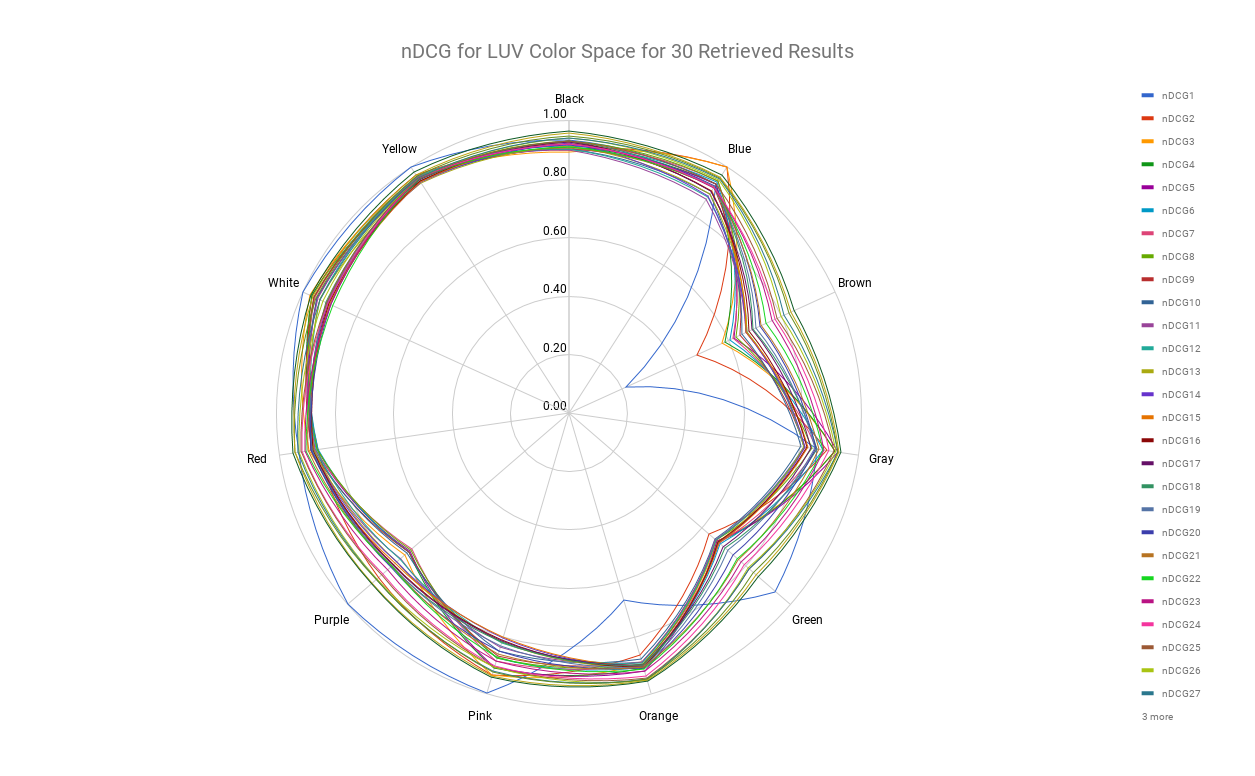
\includegraphics[width=0.9\linewidth]{image/retrievalTwo/radar_ndcg_luv.png}\\
    (a) \textit{nDCG} visualised in Radar Chart \\
    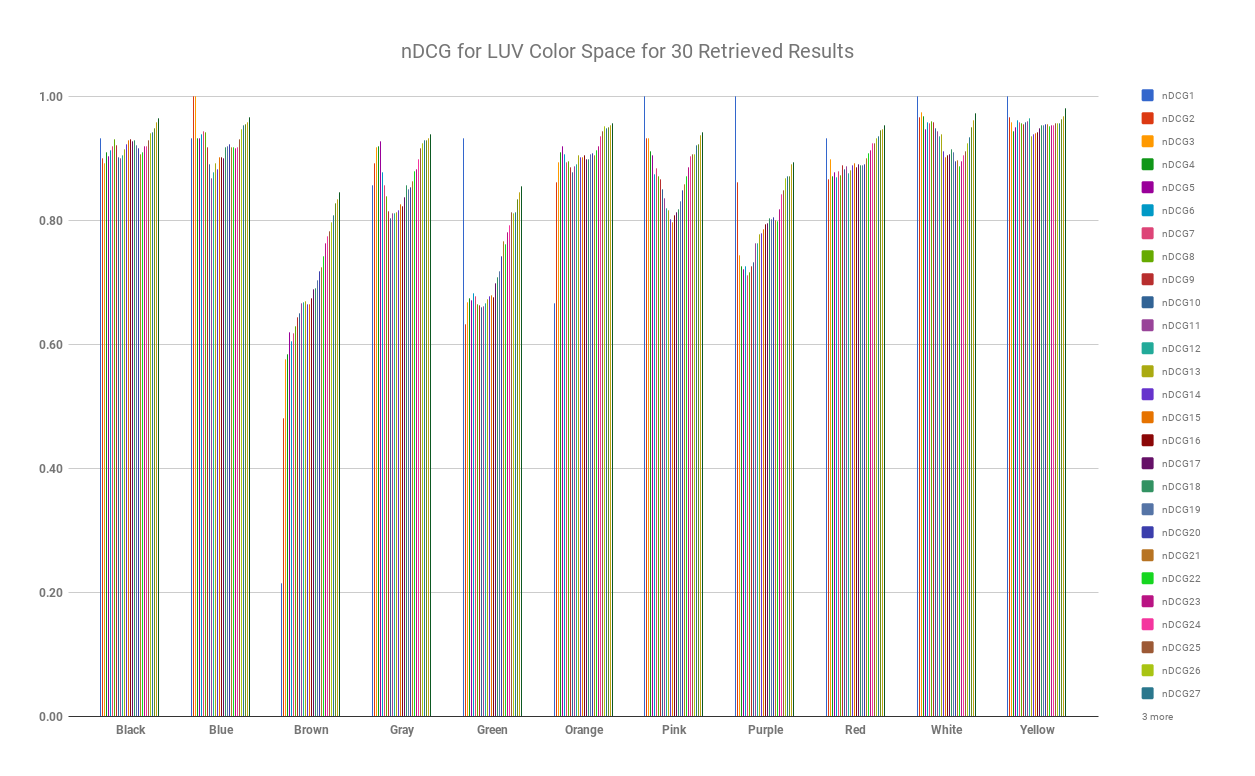
\includegraphics[width=0.9\linewidth]{image/retrievalTwo/bar_ndcg_luv.png}\\
    (b) \textit{nDCG} visualised in Bar Chart \\
  \end{tabular}
  \caption{\textit{nDCG} of the LUV Colour Mode using Radar and Bar Chart}
  \label{fig:colorndcg}
\end{figure}
\begin{table}[tb!]
	\centering
	\caption{Per-class Normalised Discounted Cumulative Gain (nDCG) based on LUV colour mode}
	\label{tab:dcgColor}
\resizebox{\textwidth}{!}{
\begin{tabular}{c||c|c|c|c|c|c|c|c|c|c|c}
& Black & Blue & Brown & Gray & Green & Orange & Pink & Purple & Red & White & Yellow \\ \hline \hline
\textit{nDCG1} & 0.93 & 0.93 & 0.21 & 0.86 & 0.93 & 0.67 & 1.00 & 1.00 & 0.93 & 1.00 & 1.00 \\
\textit{nDCG2} & 0.90 & 1.00 & 0.48 & 0.89 & 0.63 & 0.86 & 0.93 & 0.86 & 0.87 & 0.97 & 0.97 \\
\textit{nDCG3} & 0.89 & 1.00 & 0.58 & 0.92 & 0.67 & 0.89 & 0.93 & 0.74 & 0.90 & 0.97 & 0.96 \\
\textit{nDCG4} & 0.91 & 0.93 & 0.58 & 0.92 & 0.68 & 0.91 & 0.91 & 0.73 & 0.87 & 0.97 & 0.94 \\
\textit{nDCG5} & 0.90 & 0.93 & 0.62 & 0.93 & 0.67 & 0.92 & 0.90 & 0.72 & 0.88 & 0.95 & 0.95 \\
\textit{nDCG6} & 0.91 & 0.94 & 0.60 & 0.88 & 0.68 & 0.91 & 0.87 & 0.73 & 0.87 & 0.96 & 0.96 \\
\textit{nDCG7} & 0.92 & 0.94 & 0.62 & 0.86 & 0.68 & 0.89 & 0.88 & 0.71 & 0.88 & 0.96 & 0.96 \\
\textit{nDCG8} & 0.93 & 0.94 & 0.63 & 0.84 & 0.66 & 0.90 & 0.87 & 0.72 & 0.87 & 0.96 & 0.96 \\
\textit{nDCG9} & 0.92 & 0.92 & 0.64 & 0.82 & 0.66 & 0.89 & 0.87 & 0.73 & 0.89 & 0.96 & 0.96 \\
\textit{nDCG10} & 0.90 & 0.89 & 0.65 & 0.80 & 0.66 & 0.88 & 0.85 & 0.73 & 0.88 & 0.95 & 0.96 \\
\textit{nDCG11} & 0.90 & 0.87 & 0.67 & 0.81 & 0.66 & 0.89 & 0.84 & 0.76 & 0.89 & 0.94 & 0.96 \\
\textit{nDCG12} & 0.90 & 0.88 & 0.67 & 0.81 & 0.67 & 0.89 & 0.82 & 0.76 & 0.88 & 0.94 & 0.96 \\
\textit{nDCG13} & 0.91 & 0.89 & 0.67 & 0.81 & 0.67 & 0.91 & 0.82 & 0.78 & 0.88 & 0.94 & 0.94 \\
\textit{nDCG14} & 0.92 & 0.88 & 0.67 & 0.82 & 0.68 & 0.90 & 0.80 & 0.78 & 0.89 & 0.91 & 0.94 \\
\textit{nDCG15} & 0.93 & 0.90 & 0.67 & 0.83 & 0.68 & 0.90 & 0.80 & 0.79 & 0.89 & 0.90 & 0.94 \\
\textit{nDCG16} & 0.93 & 0.90 & 0.68 & 0.82 & 0.68 & 0.90 & 0.81 & 0.79 & 0.89 & 0.90 & 0.94 \\
\textit{nDCG17} & 0.93 & 0.90 & 0.69 & 0.84 & 0.70 & 0.90 & 0.81 & 0.80 & 0.89 & 0.91 & 0.95 \\
\textit{nDCG18} & 0.93 & 0.92 & 0.69 & 0.86 & 0.71 & 0.90 & 0.82 & 0.80 & 0.89 & 0.91 & 0.95 \\
\textit{nDCG19} & 0.92 & 0.92 & 0.70 & 0.85 & 0.72 & 0.91 & 0.83 & 0.80 & 0.89 & 0.91 & 0.95 \\
\textit{nDCG20} & 0.92 & 0.92 & 0.72 & 0.85 & 0.74 & 0.91 & 0.85 & 0.80 & 0.89 & 0.89 & 0.96 \\
\textit{nDCG21} & 0.91 & 0.92 & 0.72 & 0.86 & 0.77 & 0.90 & 0.86 & 0.80 & 0.90 & 0.90 & 0.95 \\
\textit{nDCG22} & 0.91 & 0.92 & 0.74 & 0.88 & 0.76 & 0.91 & 0.87 & 0.80 & 0.91 & 0.89 & 0.95 \\
\textit{nDCG23} & 0.92 & 0.92 & 0.76 & 0.88 & 0.78 & 0.92 & 0.89 & 0.82 & 0.91 & 0.90 & 0.95 \\
\textit{nDCG24} & 0.92 & 0.92 & 0.77 & 0.90 & 0.79 & 0.94 & 0.90 & 0.84 & 0.92 & 0.90 & 0.95 \\
\textit{nDCG25} & 0.93 & 0.93 & 0.78 & 0.92 & 0.81 & 0.94 & 0.91 & 0.85 & 0.93 & 0.91 & 0.96 \\
\textit{nDCG26} & 0.94 & 0.95 & 0.80 & 0.92 & 0.81 & 0.95 & 0.91 & 0.87 & 0.93 & 0.93 & 0.96 \\
\textit{nDCG27} & 0.94 & 0.95 & 0.81 & 0.93 & 0.81 & 0.95 & 0.92 & 0.87 & 0.94 & 0.93 & 0.96 \\
\textit{nDCG28} & 0.95 & 0.96 & 0.83 & 0.93 & 0.83 & 0.95 & 0.92 & 0.87 & 0.95 & 0.95 & 0.96 \\
\textit{nDCG29} & 0.96 & 0.96 & 0.83 & 0.93 & 0.85 & 0.95 & 0.94 & 0.89 & 0.95 & 0.96 & 0.97 \\
\textit{nDCG30} & 0.96 & 0.97 & 0.85 & 0.94 & 0.85 & 0.96 & 0.94 & 0.89 & 0.95 & 0.97 & 0.98 \\
\end{tabular}}
\end{table}

\subsubsection{Retrieval Speed}

The speed in which a retrieval engine returns the results plays an important role in determining the feasibility and practicality of the proposed method in real-world applications. In this experiment, the relevance of each result is not taken into consideration. Instead, the computation time taken to perform the queries were measured. The proposed method was rigorously tested with with the following criterion set: (i) Retrieval result size (recall quantity), (ii) Trajectory length, (iii) Number of colours used in the retrieval process, and (iv) Size of the top sorted color matches (to be known from hereon as `SortColourSize'). The baseline (BL) measurement takes in an input trajectory of 10 atoms, retrieving 30 results with all (11) colours considered and a SortColourSize of 200.
%Using the BL setting, the proposed method ignores all colour information during the retrieval process as only the trajectory information along with the time and date input affects the final results.

Table \ref{tab:retrievalspeed} summarises the retrieval speed of the proposed method using various settings. The collection of results was done by repeating and averaging over 20 executions of queries. From the results of the BL highlighted in the table, it is observed that the BL settings achieved an average of about 1.24 seconds when retrieving 30 results given an input trajectory of 10 atom length. The results also shows that increasing the number of displayed results does not heavily affect the processing time. However, it is noticeable that the length of input trajectory affects the processing speed more than the number of displayed results. This is consistent with the formulation of the Chamfer Distance (in Eq. \ref{eq:chamferDistance}). As the length of the input increases, the proposed method requires more time to run through all possible trajectories within the set.

To further test the retrieval speed, more precise colour information was selected as additional input query. The proposed method took considerably more time than the BL measurement which accepted vehicles of any colour. This is because the proposed method had to compare more data and sort the results in accordance to both the colour semantic as well as the similarity between the input trajectory and the database of trajectories. Similarly, when the number of desired colours increased from 1 to 5, the retrieval engine took an additional 0.3 seconds on average to process the results.

Next, to further validate the performance of the proposed method, synthetic data was generated to simulate 6 months of valid data within the database. When the BL settings were applied, the proposed method took 7.7 seconds to retrieve the results. The scalability of our semantics is significant: additional colour queries only took an extra 0.6 seconds for the retrieval of results. Furthermore, the combination of input trajectory length of 30 with 5 colour queries only took about 9.4 seconds on average using the proposed method, which is reasonably practical. When compared against traditional manual filtering and procuring of relevant results from the data, the proposed method showed significant ability to perform this to human level without compromising on the quality of results. %Without a doubt, the proposed solution is able to outperform any human. 
The comparison between the proposed method against the method proposed by \citeA{castanon2016retrieval} is shown in Table \ref{tab:compareresult}. Given the difference in the dataset used (as well as likely, different computational capabilities as well), it is difficult to direclty compare the methods used. Even though the proposed method was not able to obtain compression rates as high as those reported in \citeA{castanon2016retrieval} by direct comparison, it was able to search through 200 hours of semantic data within just 1.2 seconds. This level of efficiency is essential for real-world applications especially when dealing with large scale datasets.
% Please add the following required packages to your document preamble:
% \usepackage[table,xcdraw]{xcolor}
% If you use beamer only pass "xcolor=table" option, i.e. \documentclass[xcolor=table]{beamer}
\begin{table}[!tb]
	\centering
	\caption{Retrieval Speed with Varying Parameters}
	\label{tab:retrievalspeed}
	\resizebox{1\textwidth}{!}{
\begin{tabular}{|c|c|c|c|c|c|}
\hline
\textbf{Data Size} & \textbf{Result Size} & \textbf{Traj. Length} & \textbf{No. of Colours} & \textbf{SortColourSize} & \textbf{Avg Retrieval Speed } \\ \hline
\multicolumn{1}{|c|}{}            & \cellcolor{yellow}30                           & \cellcolor{yellow}10                         & \cellcolor{yellow}11                         & \cellcolor{yellow}200                     & \cellcolor{yellow}1246.7720 ms (BL)                        \\ \cline{2-6}
\multicolumn{1}{|c|}{}            & 30                           & 10                         & 1                         & 200                     & 1382.6237 ms                             \\ \cline{2-6}
\multicolumn{1}{|c|}{}            & 30                           & 30                         & 11                         & 200                     & 1301.3777  ms                           \\ \cline{2-6}
\multicolumn{1}{|c|}{}            & 100                          & 10                         & 11                         & 200                     & 1282.0485 ms                            \\ \cline{2-6}
\multicolumn{1}{|c|}{}            & 30                           & 10                         & 11                         & 500                     & 1374.3655 ms                             \\ \cline{2-6}
\multicolumn{1}{|c|}{}            & 30                           & 10                         & 1                          & 500                     & 1580.7543 ms                            \\ \cline{2-6}
\multicolumn{1}{|c|}{}            & 30                           & 30                         & 1                          & 500                     & 1641.2180 ms                            \\ \cline{2-6}
\multicolumn{1}{|c|}{\multirow{-8}{*}{1 month}}            & 30                           & 10                         & 5                          & 500                     & 1972.2770 ms                            \\ \hline \hline
\multicolumn{1}{|c|}{}           & \cellcolor{yellow}30                           & \cellcolor{yellow}10                         & \cellcolor{yellow}11                         & \cellcolor{yellow}200                     & \cellcolor{yellow}7745.1803 ms                            \\ \cline{2-6}
\multicolumn{1}{|c|}{}          & 30                           & 10                         & 1                          & 200                     & 7874.1965 ms                            \\ \cline{2-6}
\multicolumn{1}{|c|}{}           & 30                           & 10                         & 5                          & 200                     & 8314.7145 ms                            \\ \cline{2-6}
\multicolumn{1}{|c|}{\multirow{-4}{*}{6 month}}           & 30                           & 30                         & 5                          & 200                     & 9369.6657 ms                            \\ \hline
\end{tabular}
}\vspace{-1em}
\end{table}

% Please add the following required packages to your document preamble:
% \usepackage[table,xcdraw]{xcolor}
% If you use beamer only pass "xcolor=table" option, i.e. \documentclass[xcolor=table]{beamer}
\begin{table}[tb!]
	\centering
	\caption{Comparison between Methods: Retrieval Speed, Compression Ratio Using Trajectory/Tracklet Features}
	\label{tab:compareresult}
	\resizebox{\textwidth}{!}{
\begin{tabular}{|l|l|l|l|l|l|}
\hline
\textbf{Method}                 & \textbf{Video Duration} & \textbf{Video Size} & \textbf{DB/Index Size} & \textbf{Compression Ratio}        & \textbf{Retrieval Speed}         \\ \hline
DP + LSH
%\citeyear{castanon2016retrieval}
& 13.8 minutes                    & 1.16 GB             & 153 KB                       & 7581\%                            & 2.9 sec*                         \\ \hline
%\citeA{castanon2016retrieval}
DP + LSH & 13.8 minutes                    & 529 MB              & 65 KB                        & \cellcolor{yellow}8138.46\% & 4.32 sec*                        \\ \hline
Proposed method                      & 200 hours                       & 33.4 GB             & 16.3 MB                      & 2049.07\%                         & \cellcolor{yellow}1.2 sec** \\ \hline
\end{tabular}}
\vspace{-0.6em}
\end{table}


\section{Summary}

In this chapter, two different semantic retrieval engines are proposed to retrieve semantics extracted in Chapter \ref{section:semanticsextraction}. Both the proposed methods implement distinctly different algorithms for the retrieval process. The \versionOneRet retrieved relevant documents based on the locality in which the data was saved while the \versionTwoRet retrieved and ranked relevant documents based on the similarity with the given input query.

Both retrieval engines reported respectable precision scores when retrieving both motion and colour semantic information. The proposed \versionTwoRet also demonstrated its ability to retrieve relevant results accurately within 1.2 seconds while organising the results in the best possible manner. As the colour semantic ios not hard-coded into one final category, the colour retrieval process showed a significant improvement over the method proposed earlier in \versionOneRet.

There are potential future directions to improve the discussed setup. In order to further improve the performance of the proposed method, a more robust colour model is still much needed. Also, the proposed method which
uses Chamfer Distance to calculate the similarity between the query input and dataset records could potentially improve by maximising the dissimilarity score for cases where none of the points intersects, or in cases where only a few points intersect with the query.

